\chapter{Elektriese stroombane}\fancyfoot[LO,RE]{Fisika: Elektrisiteit en Magnetisme}

\section{Potensiaalverskil en emk}

Wanneer 'n stroombaan volledig verbind is kan lading deur die stroombaan
beweeg. Lading sal egter nie beweeg tensy daar 'n rede voor is nie, 'n krag dryf lading om die stroombaan. Dink daaraan asof 'n lading in rus is en iets
moet dit rondstoot. Dit beteken dat arbeid verrig moet word om lading te
beweeg. 'n Krag werk in op die lading en verrig arbeid om die lading te beweeg.
Die krag word voorsien deur die battery in die stroombaan.

'n Battery het die potensiaal om ladings om 'n geslote stroombaan te dryf. Die
battery het potensi\"ele energie wat omgeskakel kan word na elektriese energie
deur arbeid te verrig op die lading in die stroombaan om dit te laat beweeg.
\chapterstartvideo{VPfqj}

\Definition{Potensiaalverskil}{Potensiaalverskil is die verskil in elektriese
potensi\"ele energie per eenheidlading tussen twee punte. Die eenhede van
potensiaalverskil is die Volt (V), wat gedefinieer word as een joule per
coulomb.\\
Hoeveelheid: Volt ($V$) \hspace{.5cm} Eenheid naam: volt \hspace{.5cm} Eenheid simbool: V  }

\subsection*{Voltmeter}
\begin{minipage}{.6\textwidth}
'n Voltmeter is 'n instrument wat gebruik word om die arbeid te meet wat nodig is om lading
tussen twee punte in 'n elektriese stroombaan te dryf. 
% This would read better in the enlish version if it was rephrased as follows: A voltmeter is an instrument 
% for measuring the work done to drive charge between two points in an electric circuit. We call this the 
% potential difference because the work done is the difference in the potential energy of the two points.

Die simbool vir 'n voltmeter is:
\begin{center}
\begin{pspicture}(-2,0)(3,3)
%\psgrid
\pnode(0,0){A} \pnode(0,3){B} \pnode(3,3){C} \pnode(3,0){D}
%\battery(A)(B){}
\circledipole[parallel,parallelnode,parallelsep=.5,labeloffset=0](A)(B){V}
%\psline(B)(C) \resistor[dipolestyle=rectangle](C)(D){} \psline(D)(A)
\end{pspicture}
% \caption{ 'n Voltmeter word in parallel in 'n stroombaan gekoppel.
% A voltmeter should be connected in parallel in a circuit.}\label{fig:p:em:ec10:voltmeter}
\end{center}
\end{minipage}
\begin{minipage}{.4\textwidth}
\begin{center}
 'n Voltmeter\\
\includegraphics[width=.6\textwidth]{photos/volts_windy__Flickr.jpg}\\
\textit{Foto deur windy\_ op Flickr.}
\end{center}
\end{minipage}

\subsection*{EMK}
\begin{minipage}{.5\textwidth}
Wanneer jy die potensiaalverskil tussen (of oor) twee pole van 'n battery
meet, is jy besig om die "elektromotoriese krag" (emk) van die battery te meet.
Dit is die maksimum hoeveelheid arbeid wat die battery kan verrig om lading van
een pool deur die stroombaan tot by die ander pool te dryf.
\end{minipage}
\begin{minipage}{.5\textwidth}
\begin{center}
\begin{pspicture}(-2,0)(3,3)
%\psgrid
\pnode(0,0){A} \pnode(0,3){B} \pnode(3,3){C} \pnode(3,0){D}
\battery(A)(B){}
\circledipole[parallel,parallelnode,parallelsep=.5,labeloffset=0](A)(B){V}
%\psline(B)(C) \resistor[dipolestyle=rectangle](C)(D){} \psline(D)(A)
\end{pspicture}
% \caption{ 'n Voltmeter word in parallel aan 'n stroombaan gekoppel
% voltmeter should be connected in parallel in a circuit.} \label{fig:p:em:ec10:voltmeter}
\end{center}
\end{minipage}

% Hierdie drywingspotensiaal is gelyk aan die totale potensi\"ele energie in die stroombaan.
% Dit beteken dat die spanning oor die battery gelyk is aan die som van die spanning in die stroombaan.
%
% Ons kan hierdie kennis gebruik om probleme op te los waar die spanning oor elke element in die stroombaan sommeer na die emk toe.
%
% This driving potential energy is equal to the total potential energy (used (Kill this word, then it reads correctly.
% Potential energy is not used.)) in the circuit.
% This means that the voltage across the battery is equal to the sum of the voltages in the circuit.
% 
% We can use this information to solve problems in which the voltages across elements in a circuit add up to the emk. 
% \begin{equation*}
% EMF = V_{Totaal}
% \end{equation*}
% 
% Ons noem die bewegende lading 'n "stroom" en ons sal later daaroor praat. Die
% hoeveelheid arbeid om 'n lading van een punt na 'n ander te beweeg word die
% potensiaalverskil genoem.
%
% We call the moving charge "current" and we will talk about this later. The
% amount of work to move a charge
% from one point to another point is called potential difference. 
%
% Die posisie van die lading in die stroombaan dui aan hoeveel potensi\"ele
% energie dit het op grond van die krag
% wat daarop inwerk. Dit is soos gravitasiekrag; hoe ho\"er 'n voorwerp bo die
% grond is, hoe ho\"er is sy potensi\"ele energie.
%
% The position of the charge in the circuit tells you how much potential energy
% it has because of the force being exerted on it. This is like the force from
% gravity, the higher an object is above the ground (position) the more
% potential energy it has.
% 
% Let op dat dit 'n verskil is tussen die waardes van die potensi\"ele energie
% by twee punte, dus s\"e ons dat die potensiaalverskil gemeet word tussen
% of oor twee punte, nie deur twee punte nie.
% Notice that it is a difference between the value of potential energy at two
% points so we say that potential difference
% is measured between or across two points. We do not say potential difference
% through something.



\IFact{Die Volt is vernoem na die Italiaanse fisikus Alessandro Volta
(1745--1827).} 

Elektriese potensiaalverskil word ook spanning genoem.

\begin{minipage}{.5\textwidth}
Wanneer jy potensiaalverskil meet oor twee pole van 'n battery \textbf{in 'n
geslote baan}, meet jy die terminaal of poolpotensiaalverskil (poolspanning)
van die battery. Al meet ons dit ook in volt, is dit nie dieselfde as die emk
nie. Die verskil is die arbeid wat verrig word om die lading deur die battery te
dryf.
\end{minipage}
\begin{minipage}{.5\textwidth}
\begin{center}
\begin{pspicture}(-2,0)(3,3)
%\psgrid
\pnode(0,0){A} \pnode(0,3){B} \pnode(3,3){C} \pnode(3,0){D}
\battery(A)(B){}
\circledipole[parallel,parallelnode,parallelsep=.5,labeloffset=0](A)(B){V}
\psline(B)(C) \resistor[dipolestyle=rectangle](C)(D){} \psline(D)(A)
\end{pspicture}
% \caption{ 'n Voltmeter word in parallel aan 'n stroombaan gekoppel.}
\label{fig:p:em:ec10:voltmeter}
\end{center}
\end{minipage}
\begin{minipage}{.5\textwidth}
\begin{center}
Batterye\\
\includegraphics[width=.8\textwidth]{photos/batterystack.jpg}\\
\textit{Fotografie op Flickr.}
\end{center} 
\end{minipage}
\begin{minipage}{.5\textwidth}
Een geleier van die voltmeter is gekoppel aan een pool van die battery en die
ander geleier is gekoppel aan die ander pool van die battery. Die voltmeter kan
ook gebruik word om die spanning oor 'n resistor of enige ander komponent van
 'n stroombaan te meet, maar moet in parallel gekoppel word.
\end{minipage}


\section{Stroom}

\subsection*{Vloei van lading}

Wanneer ons praat van stroom, dan praat ons van die hoeveel ladings wat by 'n vaste punt
in 'n stroombaan verby beweeg in een sekonde. Dink daaraan dat ladings deur die
battery rondgestoot word in die stroombaan. Daar is ladings in die geleiers,
maar sonder die battery sal hulle nie beweeg nie.\\
\mindsetvid{Meet van stroom in 'n stroombaan.}{VPfva}
\begin{minipage}{.5\textwidth}
Wanneer een lading beweeg, dan beweeg die een langs hom ook. Hulle hou hulle
afstande soos albasters in 'n pyp, soos in die skets.
\begin{center}
\scalebox{.7}{
\begin{pspicture}(-1.6,-0.4)(6.8,0.4)
%\psgrid[gridcolor=gray]
\psline(0,0)(5,0) \psline(0,0.4)(5,0.4)
\multirput(0.4,0.2)(0.4,0){12}{\pscircle*(0,0){0.2}} \rput(-1,0){
\pscircle*(0,0.25){0.2} \uput[d](0,0.2){albaster} }\rput(6.2,0){
\pscircle*(0,0.25){0.2} \uput[d](0,0.2){albaster} }
\psline{->}(-0.6,0.2)(0,0.2) \psline{->}(5.2,0.2)(5.8,0.2)
\end{pspicture}}
\end{center}
As jy een albaster in die pyp stoot, moet daar een uitkom aan die anderkant van
die pyp. Dit is soortgelyk aan die lading in die geleiers van 'n stroombaan. As
een lading beweeg, dan beweeg almal en dieselfde aantal beweeg op elke punt in
die stroombaan. Hierdie is as gevolg van die behoud van lading wat ons alreeds
behandel het in \textsl{Elektrostatika}.
 \end{minipage}
\begin{minipage}{.5\textwidth}
\begin{center}
\textbf{Koperdraad}\\
\includegraphics[width=.8\textwidth]{photos/copperwire.jpg}\\
\textit{Foto op Flickr.}
\end{center}  
\end{minipage}
\IFact{Benjamin Franklin het 'n aanname gemaak oor die rigting van die stroom
wanneer gladde was met growwe wol gevryf word. Hy het gedink die ladings vloei
van die was na die wol (d.i. van positief na negatief), wat die teenoorgestelde
is van die werklike rigting. As gevolg hiervan word ges\^e dat elektrone
\emph{negatiewe} lading het so het alle voorwerpe wat Ben Franklin ''negatief''
genoem het, eintlik 'n oormaat elektrone. Teen die tyd dat die ware rigting van
elektronvloei ontdek is, was die konvensie van ''positief'' en ''negatief''
alreeds so gevestig in die wetenskaplike w\^ereld dat daar nie moeite gedoen is om
dit te verander nie.}
\Definition{Stroom}{Stroom is die tempo waarteen ladings by 'n vaste punt
in 'n stroombaan verby beweeg. Die eenheid van stroom is die ampere, wat
gedefinieer word as een coulomb per sekonde.\\
Hoeveelheid: Stroom ($I$) \hspace{.5cm} Eenheid naam: ampere \hspace{.5cm} Eenheid simbool: A  }
Ons gebruik die simbool $I$ om stroom aan te dui en dit word in ampere
(A) gemeet. Een ampere is een coulomb lading wat in een sekonde verby beweeg.
($\text{C} \cdot \text{s}^{-1}$).
\begin{equation*}
\boxed{I = \frac{Q}{\Delta t}}
\end{equation*}
\begin{minipage}{.5\textwidth}
\begin{center}
\textbf{Plasmabal}\\
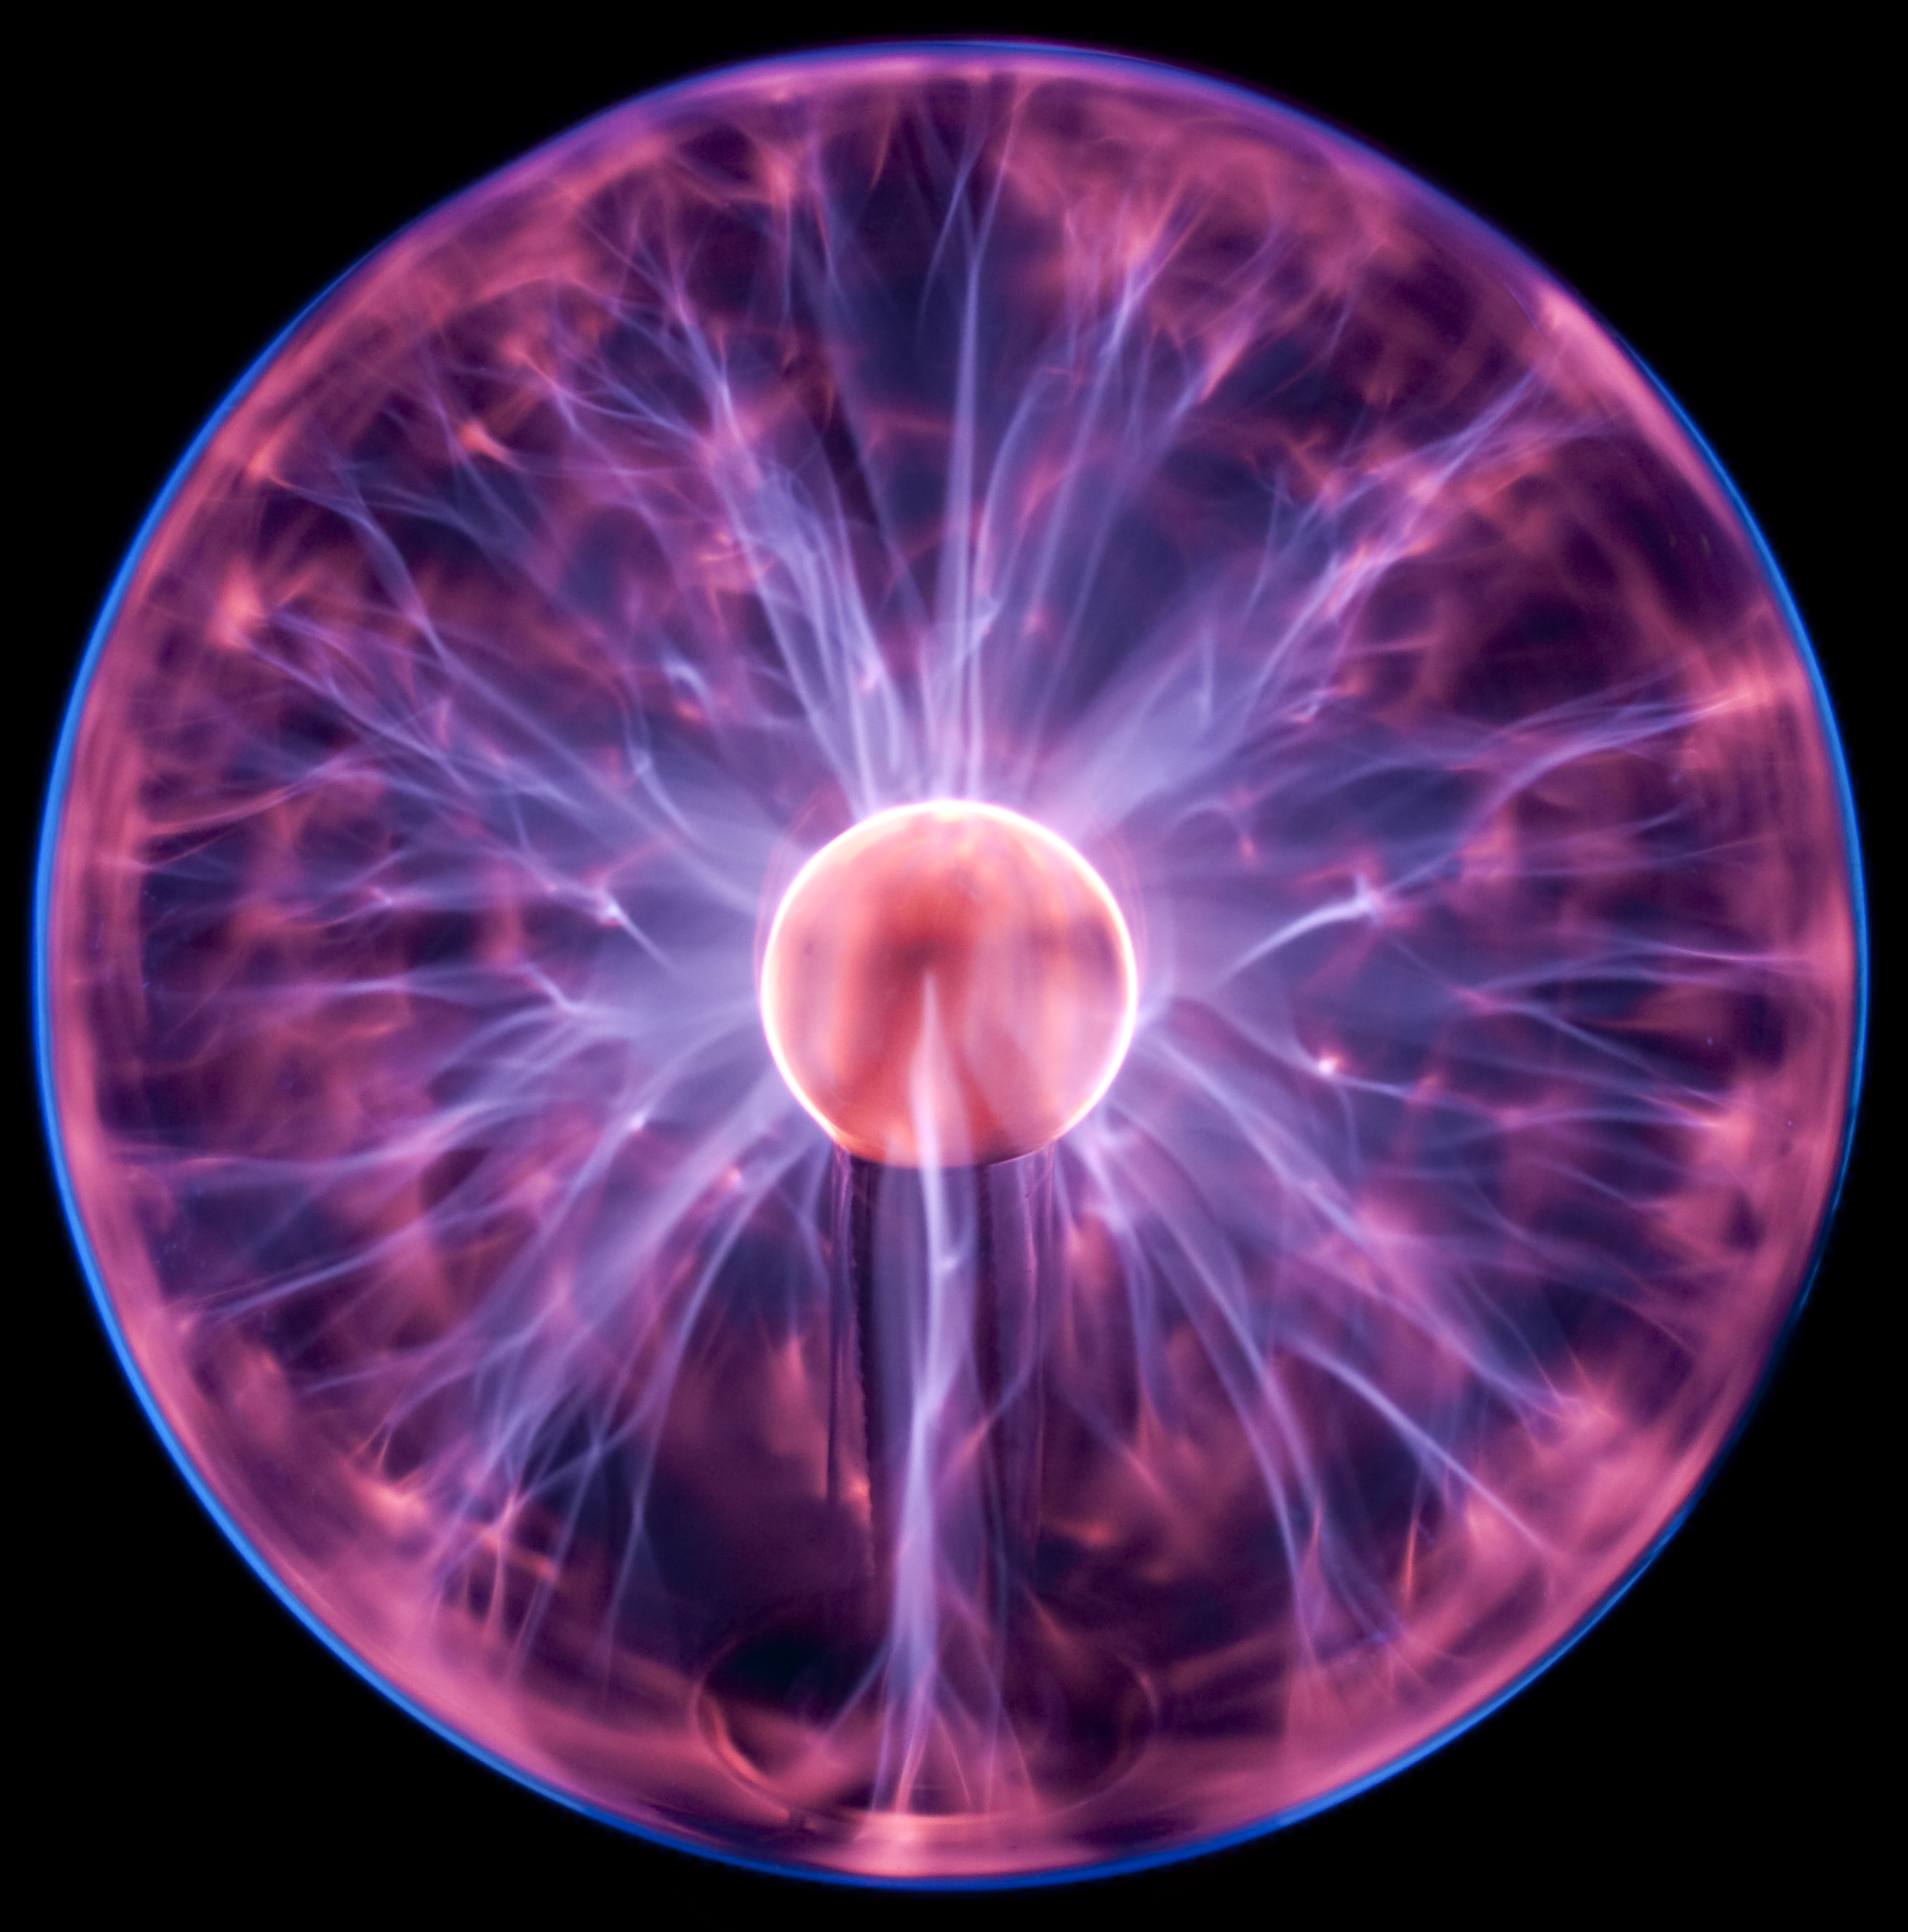
\includegraphics[width=.8\textwidth]{photos/plasmaball_by_ahisgett.jpg}\\
\textit{Foto deur ahisgett op Flickr.}
\end{center}   
\end{minipage}
\begin{minipage}{.5\textwidth}

Wanneer stroom in 'n stroombaan vloei dui ons dit aan in 'n diagram deur
pyltjies by te voeg. Die pyltjies dui die rigting van die
stroom in 'n stroombaan aan. Per konvensie s\^e ons die stroom vloei vanaf die
positiewe pool van die battery na die negatiewe pool.

As die spanning hoog genoeg is kan stroom deur byna enigiets vloei. In die
plasmabal links word 'n hoog genoeg spanning geskep om lading deur die gas in
die bal te laat vloei. Die spanning is hoog maar die resulterende stroom is
laag. Dit maak dit veilig om aan te raak.
\end{minipage}


\subsection*{Ammeter}

\begin{minipage}{.5\textwidth}
 'n Ammeter is 'n instrument wat gebruik word om die vloeitempo van elektriese
stroom in 'n stroombaan te meet. Aangesien ons belangstel om die stroom
\textit{deur} 'n komponent te meet, moet die ammeter in \textit{serie} met die
gemete komponent gekoppel word.
\begin{center}
\scalebox{.8}{
\begin{pspicture}(0,0)(3,3)
%\psgrid
\pnode(0,0){A} \pnode(0,2.5){B} \pnode(3,2.5){C} \pnode(3,0){D}
\battery[tension,dipoleconvention=generator](A)(B){$I$} \circledipole[labeloffset=0](B)(C){A}
\resistor[intensity,dipolestyle=rectangle](D)(C){} \wire[tension,arrowscale=2](D)(A)
\end{pspicture}}
\label{fig:p:em:ec10:ammeter}
\end{center}
\end{minipage}
\begin{minipage}{.5\textwidth}
\begin{center}
\textbf{Ammeter}\\
%\includegraphics[width=.8\textwidth]{photos/ammeter_by_Hillwalker-ca_flickr.jpg}\\
%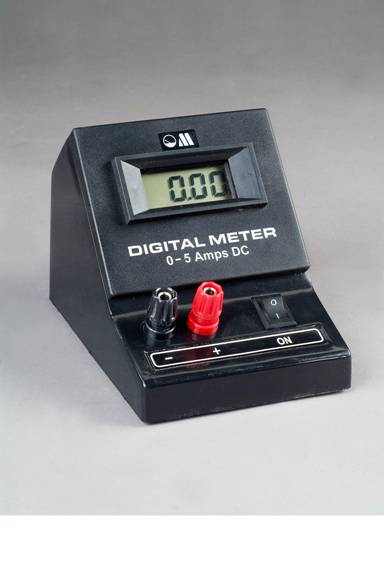
\includegraphics[width=.8\textwidth]{photos/type2ammeter.jpg}\\
\includegraphics[width=.6\textwidth]{photos/ammeter.jpg}\\
%\textit{Photography by Hillwalker-ca on Flickr.com}
\end{center}  
\end{minipage}

\begin{activity}{Bou van stroombane}
%\begin{minipage}{.5\textwidth}
Bou stroombane om die emk en die poolspanning van 'n battery te meet.

% \end{minipage}
% \begin{minipage}{.5\textwidth}
%\subsubsection*{Components of electrical circuits}
Algemene elemente (komponente) wat in stroombane aangetref word sluit in
gloeilampe, batterye, geleiers, skakelaars, resistors, voltmeters en ammeters.
Jy het alreeds baie hiervan geleer. Hieronder is 'n tabel met die items en
hulle simbole:

\begin{table}[H]
\begin{center}
\begin{tabular}{|l|c|l|}\hline
\textbf{Komponent} & \textbf{Simbool} & \textbf{Gebruik} \\\hline\hline
\raisebox{0.35cm}{gloeilamp}&\begin{pspicture}(-0.5,-0.5)(0.5,0.5)
\scalebox{0.75}{\lamp(-1,0)(1,0){}}\end{pspicture} & 
\raisebox{0.35cm}{gloei wanneer lading daardeur beweeg} \\ \hline
\raisebox{0.35cm}{battery}&\begin{pspicture}(-0.5,-0.5)(0.5,0.5)
\scalebox{0.75}{\battery(-1,0)(1,0){}}\end{pspicture} & 
\raisebox{0.35cm}{verskaf energie vir ladings om te beweeg} \\ \hline
\raisebox{0.35cm}{skakelaar}&\begin{pspicture}(-0.5,-0.5)(0.5,0.5)
\scalebox{0.75}{\switch(-1,0)(1,0){}}\end{pspicture} & 
\raisebox{0.35cm}{maak 'n stroombaan oop of toe} \\ \hline
\raisebox{-0.35cm}{resistor}&\begin{pspicture}(-0.5,0)(0.5,0.5)
\scalebox{0.75}{\resistor(-1,0)(1,0){}}\end{pspicture} & 
\raisebox{-0.35cm}{bied weerstand teen die vloei van lading} \\ 
&
OF& \\ 
&
\begin{pspicture}(-0.75,-0.25)(0.75,0.25)
\scalebox{0.75}{\resistor[dipolestyle=zigzag](-1,0)(1,0){}}\end{pspicture} & \\
\hline
\raisebox{0.35cm}{voltmeter}&\begin{pspicture}(-0.5,-0.5)(0.5,0.5)
\scalebox{0.75}{\circledipole[labeloffset=0](-1,0)(1,0){V}}\end{pspicture} & 
\raisebox{0.35cm}{meet potensiaalverskil} \\ \hline
\raisebox{0.35cm}{ammeter}&\begin{pspicture}(-0.5,-0.5)(0.5,0.5)
\scalebox{0.75}{\circledipole[labeloffset=0](-1,0)(1,0){A}}\end{pspicture} & 
\raisebox{0.35cm}{meet die stroom in 'n stroombaan} \\ \hline
\raisebox{0.35cm}{geleier}&\begin{pspicture}(0,0)(1,1)
\psline(-0.25,0.5)(1.25,0.5)\end{pspicture} & 
\raisebox{0.35cm}{koppel stroombaan-elemente} \\ \hline
\hline
\end{tabular}
\end{center}
\end{table}
Eksperimenteer met verskillende kombinasies van komponente in stroombane.

%\end{minipage}
\end{activity}
\Tip{ 'n Battery verskaf \textbf{nie} dieselfde stroom ongeag wat daaraan
gekoppel is \textbf{nie}. Die spanning bly konstant, maar die stroom wissel na
gelang van wat in die stroombaan is.}

Die tabel hieronder gee 'n opsomming van die gebruike van elke meetinstrument
wat ons bespreek het en toon die wyse van koppeling aan 'n
stroombaan-komponent.

\begin{center}
\begin{tabular}{ | c | c | c | }
\hline 
\textbf{Instrument} & \textbf{Gemete grootheid} & \textbf{Korrekte koppeling}
\\ \hline \hline 
Voltmeter & Spanning & in Parallel \\ \hline Ammeter &
Stroom & in Serie \\ \hline
\hline
\end{tabular}
\end{center}


\begin{activity}{Gebruik van meters}

Indien moontlik, koppel meters in stroombane om vertroud te raak met die
gebruik van meters om elektriese hoeveelhede te meet. Waar die meters meer as
een skaal het, gebruik altyd die \textbf{grootste skaal} eerste sodat jy nie
die meter beskadig deur die meter se grens te oorskry nie.
\end{activity}



\begin{wex}{Berekening van stroom I}
{ 'n Hoeveelheid lading van 45 C beweeg verby 'n punt in 'n stroombaan in 1
sekonde. Wat is die stroom in die baan?
}{%
\westep{Analiseer die vraag}

Ons word 'n hoeveelheid lading en 'n tyd gegee en gevra om die stroom te
bereken. Ons weet die stroom is die tempo waarteen lading by 'n vaste punt in
 'n stroombaan verby beweeg, dus het ons al die inligting wat ons benodig. Ons
het die hoeveelhede reeds in die regte eenhede.
\westep{Toepassing van die beginsels}
Ons weet dat:
\begin{eqnarray*}
I &=& \frac{Q}{\Delta t} \\
I &=& \frac{45~\text{C}}{1~\text{s}} \\
I &=& 45~\text{C} \cdot \text{s}^{-1} \\
I &=& 45~\text{A} \\
\end{eqnarray*}
\westep{Skryf die finale resultaat neer}
Die stroom is 45~A.
}
\end{wex}

\begin{wex}{Berekening van die stroom II}
{ 'n Lading van 53 C beweeg verby 'n vaste punt in 2 sekondes. Wat is die stroom
in die stroombaan?
}{%
\westep{Analiseer die vraag}
Die lading en die tyd is aan ons gegee en ons word gevra om die stroom te
bereken. Ons weet die stroom is die tempo waarteen lading by 'n vaste punt in
 'n stroombaan verby beweeg, dus het ons al die inligting wat ons benodig. Ons
het die hoeveelhede reeds in die regte eenhede.
\westep{Toepassing van die beginsels}
Ons weet dat:
\begin{eqnarray*}
I &=& \frac{Q}{\Delta t} \\
I &=& \frac{53~\text{C}}{2~\text{s}} \\
I &=& 26,5~\text{C} \cdot \text{s}^{-1} \\
I &=& 26,5~\text{A} \\
\end{eqnarray*}
\westep{Skryf die finale resultaat neer}
Die stroom is 26,5~A.
}
\end{wex}

\begin{wex}{Berekening van die stroom III}
{95 elektrone beweeg verby 'n vaste punt in 'n stroombaan in een tiende van 'n
sekonde. Wat is die stroom in die baan?
}{%
\westep{Analiseer die vraag}
Die aantal gelaaide deeltjies wat verby 'n vaste punt beweeg en die tyd wat
dit neem is aan ons gegee. Ons weet dat die stroom die tempo is waarteen
deeltjies by 'n vaste punt verby beweeg, dus moet ons die lading bereken. In die
vorige hoofstuk het ons geleer dat die lading wat deur een elektron gedra word
is $1,6\times10^{-19}~\text{C}$.
\westep{Toepassing van beginsels: bepaal die lading}
Ons weet dat een elektron 'n lading dra van $1,6\times10^{-19}~\text{C}$,
dus is die totale lading:
\begin{eqnarray*}
Q & = & 95 \times 1,6\times10^{-19}~\text{C} \\
& = & 1,52\times10^{-17}~\text{C} 
\end{eqnarray*}
\westep{Toepassing van beginsels: bepaal die lading}
Ons weet dat:
\begin{eqnarray*}
I &=& \frac{Q}{\Delta t} \\
I &=& \frac{1,52\times10^{-17}~\text{C}}{\frac{1}{10}~\text{s}} \\
I &=&
\frac{1,52\times10^{-17}~\text{C}}{1}\times{\frac{1}{{\frac{1}{10}~\text{s}}}}
\\
I &=& \frac{1,52\times10^{-17}~\text{C}}{1}\times\frac{10}{1~\text{s}} \\
I &=& 1,52\times10^{-16}~\text{C} \cdot \text{s}^{-1} \\
I &=& 1,52\times10^{-16}~\text{A} \\
\end{eqnarray*}
\westep{Skryf die finale resultaat neer}
Die stroom is $1,52\times10^{-16}$~A.
}
\end{wex}


\section{Weerstand}

Weerstand is 'n mate van ``hoe moeilik'' dit is om elektrisiteit deur 'n
stroombaan-element te ``stoot.'' Weerstand is ook van toepassing op 'n totale
stroombaan.
\mindsetvid{weerstand}{VPfvk}
\subsection*{Wat veroorsaak weerstand?}

\begin{minipage}{.5\textwidth}
Op 'n mikroskopiese vlak bots elektrone wat deur 'n geleier beweeg met die
deeltjies waaruit die geleier bestaan. Wanneer hulle bots (of interaksie
plaasvind), dra hulle kinetiese energie oor. Die elektrone verloor dus energie
en beweeg stadiger. Dit lei tot weerstand. Die energie wat oorgedra word
veroorsaak dat die resistor warm word.
Jy kan dit direk voel deur aan 'n selfoonlaaier te raak terwyl dit 'n selfoon
laai - die laaier word warm want sy stroombane het resistors in!
\end{minipage}
\begin{minipage}{.5\textwidth}
\begin{center}
 Voorbeelde van resistors\\
\includegraphics[width=.8\textwidth]{photos/resistors_oskay.jpg}\\
\textit{Foto deur oskay op Flickr}
\end{center}
\end{minipage}

\Definition{Weerstand}{Weerstand maak die vloei van ladings in 'n
stroombaan stadiger. Die eenhede van weerstand is die ohm ($\Omega$) wat
gedefinieer word as 'n volt per ampere stroom.\\
Hoeveelheid: Weerstand ($R$) \hspace{.5cm} Eenheid naam: ohm \hspace{.5cm} Eenheid simbool: $\Omega$   }
\begin{equation*}
1 \ \text{Ohm} = 1 \frac{\text{Volt}}{ \text{Ampere}}
\end{equation*}

\IFact{Fluoresserende ligte gebruik nie dun drade nie; hulle gebruik die
eienskap dat sekere gasse gloei wanneer 'n stroom deur hulle vloei. Hulle is
baie meer effektief (baie minder weerstand) as gloeilampe.} 

\begin{minipage}{.5\textwidth}
\begin{center}
Gloeilamp filament\\
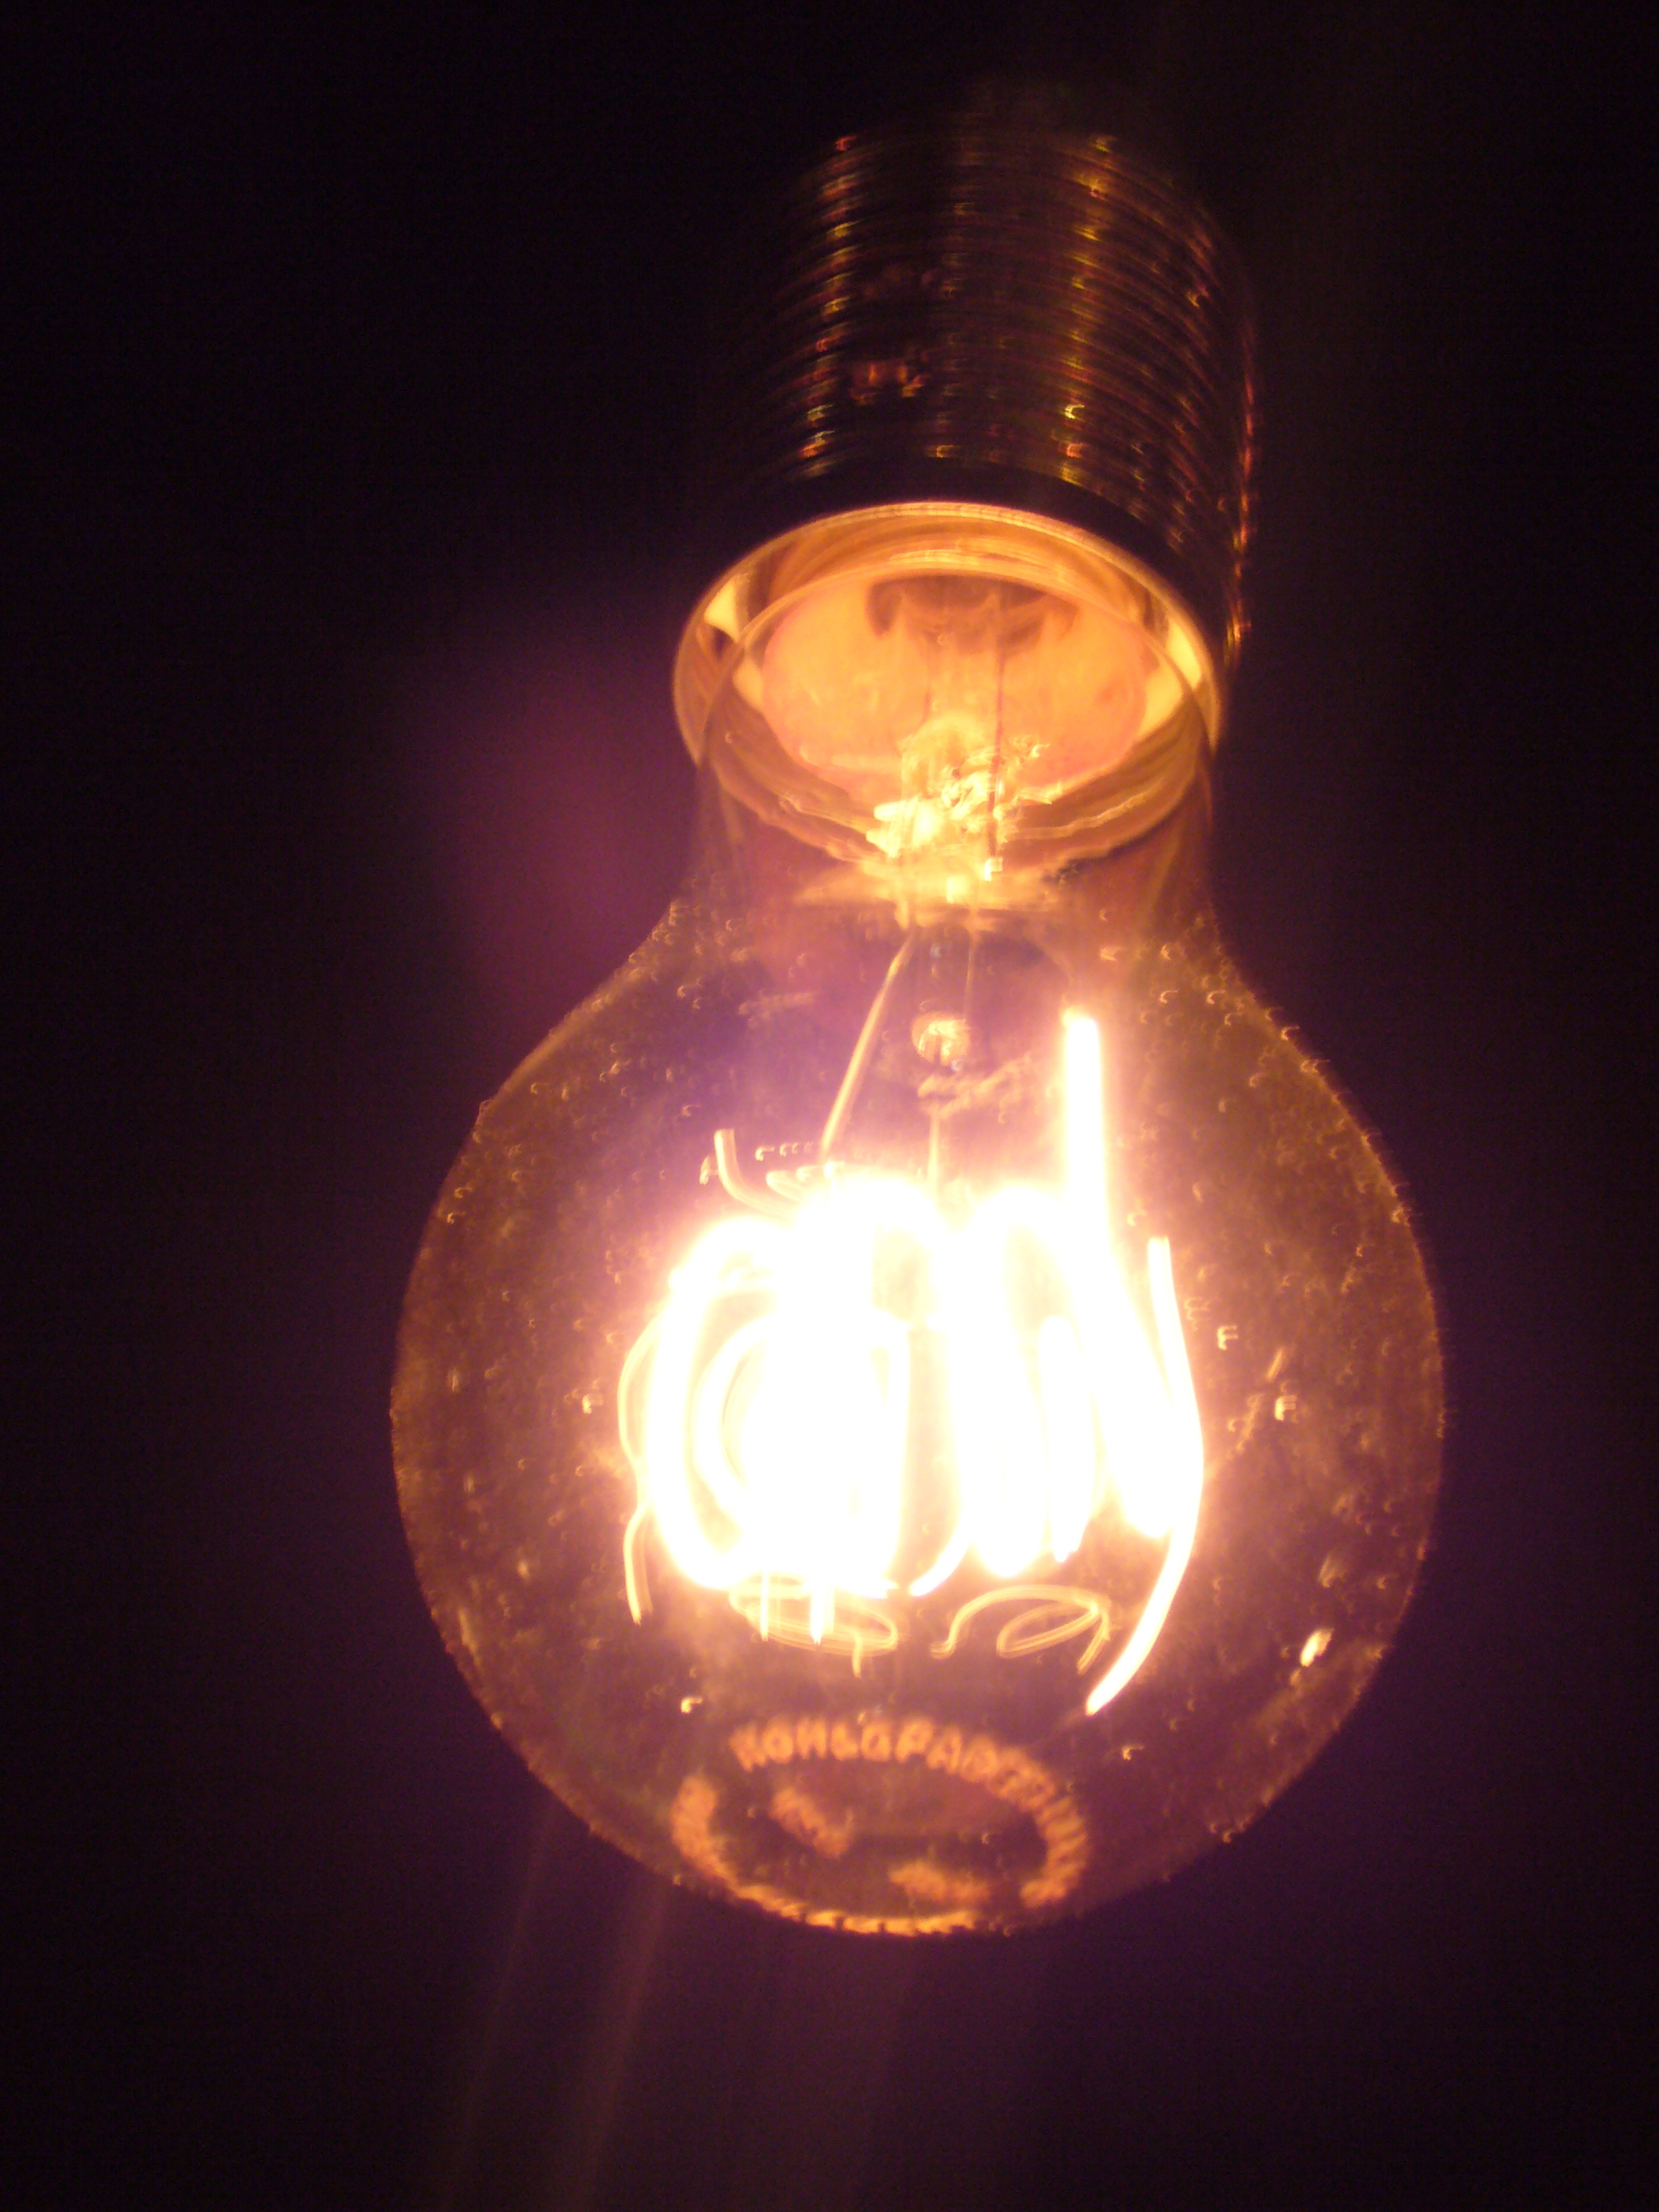
\includegraphics[width=.55\textwidth]{photos/lightbulb_by_clagnut.jpg}\\
\textit{Foto deur clagnut op Flickr.}
\end{center}  
\end{minipage}
\begin{minipage}{.5\textwidth}

\textit{Alle} geleiers het weerstand. Byvoorbeeld, 'n stuk draad het
minder weerstand as 'n gloeilamp, maar beide het weerstand. \\

 'n Gloeilamp is 'n baie dun draadjie in 'n glasomhulsel. Die ho\"e weerstand van
die dun draadjie (filament) in 'n gloeilamp veroorsaak dat die elektrone 'n
groot hoeveelheid van hulle kinetiese energie oordra in die vorm van hitte.
Hierdie hitte is genoeg om die filament witwarm te laat gloei, wat lig afgee.

\end{minipage}

Die drade wat die lamp koppel aan die sel of battery word amper glad nie warm
nie al dra dit dieselfde stroom. Dit is as gevolg van hulle veel laer
weerstand op grond van hulle veel groter deursnit (hulle is dikker).

 'n Belangrike effek van 'n resistor is dat dit elektriese energie
\textit{omskakel} na ander vorms van \textbf{hitte}-energie.
\textbf{Ligenergie} is 'n neweproduk van die hitte wat opgewek word.

\IFact{Daar is 'n spesiale tipe geleier, genoem 'n \textbf{supergeleier}, wat
geen weerstand het nie, maar die materiale van alle supergeleiers begin eers
supergeleiding te toon by baie lae temperature. Die ``hoogste'' temperatuur
supergeleier is kwik\-ba\-ri\-um\-kal\-si\-um\-ko\-per\-ok\-sied (HgBa$_2$Ca$_2$Cu$_3$O$_x$),
wat supergelei by temperature van -140$^{o}$~C en kouer.}

\subsubsection{Fisiese eienskappe wat weerstand be\"invloed}

Die fisiese eienskappe van 'n resistor be\"invloed sy totale weerstand.
\begin{itemize}
 \item \textbf{Lengte}: As 'n resistor langer word, word sy weerstand groter.
As jy die lengte van 'n resistor vergroot met 'n sekere faktor sal die
weerstand vergroot met dieselfde faktor.
\item \textbf{Wydte en hoogte of deursnitarea}: As 'n resistor 'n groter pad
verskaf deur wyer of bre\"er gemaak te word kan meer stroom daardeur vloei. As
die totale oppervlak waardeur die stroom vloei (deursnitarea) vergroot word
met 'n sekere faktor, word die weerstand met dieselfde faktor laer .
\end{itemize}
\textbf{Uitbreiding:} Vir 'n enkele resistor kan dit soos volg opgesom word:
\begin{equation*}
 R\propto\frac{L}{A},
\end{equation*} waar $L$ die lengte en $A$ die deursnitarea is.

\subsubsection*{Hoekom word batterye pap?}
 'n Battery stoor chemiese energie. Wanneer dit in 'n stroombaan gekoppel word
vind daar 'n chemiese reaksie binne die battery plaas wat chemiese
potensi\"ele energie omskakel na elektriese energie. Hierdie elektriese energie
verskaf krag aan die elektrone om deur die stroombaan te beweeg. Al die
stroombaan-elemente (soos geleiers, resistors en gloeilampe) bied 'n mate van
weerstand teen die vloei van lading en skakel die elektriese energie om na
hitte en in die gloeilamp se geval, lig.
Aangesien energie altyd behoue bly, sal die battery pap wees wanneer al sy
chemiese energie omgeskakel is na ander vorme van energie.

\subsection*{Resistors in elektriese stroombane}
Dit is belangrik om te verstaan wat die effek van die byvoeging van
resistors in 'n stroombaan op die \textit{totale} weerstand van die baan is en
op die stroom wat in die baan kan vloei.


\section{Potensiaalverskil en resistors in serie}

\begin{mdframed}
Wanneer ons resistors in serie in 'n stroombaan sit: 
\begin{itemize}
 \item is daar net een pad waarin die stroom kan vloei, dus \textbf{is die stroom dieselfde op elke punt in die stroombaan}.
 \item die potensiaalverskil word \textbf{gedeel} oor die resistors. Die potensiaal oor die battery in die stroombaan is gelyk aan die som van die resistors in serie.
\begin{equation*}
 \boxed{V_{battery}=V_1+V_2+\ldots}
\end{equation*}
\item Die weerstand teen die vloei van die stroom \textbf{vermeerder}. Die totale weerstand, $R_S$ word gegee deur:
\begin{equation*}
 \boxed{R_S = R_1+R_2+\ldots}
\end{equation*}
\end{itemize}
\end{mdframed}

Ons sal elkeen van hierdie eienskappe van serie stroombane in meer detail bestudeer.

Wanneer daar resistors in serie is, een na die ander, is daar 'n
potensiaalverskil oor elke resistor. Die totale potensiaalverskil oor 'n
versameling resistors in serie is die som van die potensiaalverskille oor
elkeen van die resistors in die versameling.
\begin{equation*}
 \box{V_{battery}=V_1+V_2+\ldots}
\end{equation*}


Beskou die stroombane hieronder. As ons die potensiaalverskille tussen al die
swart kolletjies in die stroombane meet, sal dit dieselfde wees as wat ons
vantevore gesien het. Ons weet dus dat die potensiaalverskil dieselfde is oor
een, twee of drie resistors. Ons weet ook dat arbeid nodig is om die lading
deur elke resistor te laat vloei.

\begin{center}
\begin{pspicture}(0,-0.5)(12,3.5)
%\psgrid
\pnode(0,0){A}
\pnode(0,3){B}
\pnode(3,3){C}
\pnode(3,0){D}
\psdot[dotscale=2](A)
\psdot[dotscale=2](B)

% draw battery and wires

\battery(A)(B){}
\psline(B)(C)
\psline(A)(D)

% draw resistors

\resistor[dipolestyle=rectangle](C)(D){}

% Second case
\rput(4,0){
% draw battery and wires
\pnode(0,0){A}
\pnode(0,3){B}
\pnode(3,3){C}
\pnode(3,0){D}

\battery(A)(B){}
\psline(B)(C)

\psdot[dotscale=2](A)
\psdot[dotscale=2](B)



% draw resistors

\resistor[dipolestyle=rectangle](C)(D){}
\resistor[dipolestyle=rectangle](A)(D){}
%\resistor[dipolestyle=rectangle](H)(J){}
}

% Third case
\rput(8,0){
% draw battery and wires
\pnode(0,0){A}
\pnode(0,3){B}
\pnode(3,3){C}
\pnode(3,0){D}
\pnode(3,2.5){E}
\pnode(3,.5){F}
\pnode(2,2.5){G}
\pnode(4,2.5){H}
\pnode(2,.5){I}
\pnode(4,.5){J}

\battery(A)(B){}

\psdot[dotscale=2](A)
\psdot[dotscale=2](B)


% draw resistors

\resistor[dipolestyle=rectangle](A)(D){}
\resistor[dipolestyle=rectangle](D)(C){}
\resistor[dipolestyle=rectangle](B)(C){}
}

\end{pspicture}
\end{center}

Kom ons beskou hierdie in meer detail. In die figuur hieronder kan jy sien wat
die gemete waardes vir elk van drie identiese resistors in serie kan wees. Die
totale spanning oor al drie resistors is die som van die spanning oor elk
van die onderskeie resistors. Resistors in serie is ook bekend as
\textbf{spanningsverdelers} omdat al die spanning oor die resistors verdeel is
oor die individuele resistors.

\begin{center}
\begin{pspicture}(0,-3.4525)(13.355,3.4325)
\psline[linewidth=0.04cm](1.88,1.3325)(1.88,0.3525)
\psline[linewidth=0.04cm](2.0,0.9725)(2.0,0.5925)
\psframe[linewidth=0.04,dimen=outer](1.14,-0.5075)(0.42,-0.8275)
\psframe[linewidth=0.04,dimen=outer](2.24,-0.5075)(1.52,-0.8275)
\psframe[linewidth=0.04,dimen=outer](3.32,-0.5075)(2.6,-0.8275)
\psline[linewidth=0.04cm](0.42,-0.6675)(0.02,-0.6675)
\psline[linewidth=0.04cm](0.02,-0.6675)(0.04,0.8525)
\psline[linewidth=0.04cm](0.04,0.8525)(1.82,0.8525)
\psline[linewidth=0.04cm](3.72,-0.6875)(3.32,-0.6875)
\psline[linewidth=0.04cm](3.7,-0.7075)(3.72,0.8125)
\psline[linewidth=0.04cm](3.72,0.8125)(2.08,0.8125)
\psline[linewidth=0.04cm](1.12,-0.6875)(1.52,-0.6875)
\psline[linewidth=0.04cm](2.22,-0.6875)(2.62,-0.6875)
\psline[linewidth=0.04cm](7.86,3.4125)(7.86,3.4125)
\psframe[linewidth=0.04,dimen=outer](7.68,0.0925)(6.96,-0.2275)
\psframe[linewidth=0.04,dimen=outer](9.4,0.0925)(8.68,-0.2275)
\psframe[linewidth=0.04,dimen=outer](11.1,0.0925)(10.38,-0.2275)
\psline[linewidth=0.04cm](7.64,-0.0675)(8.68,-0.0675)
\psline[linewidth=0.04cm](9.38,-0.0675)(10.42,-0.0675)
\psline[linewidth=0.04cm](6.96,-0.0675)(6.46,-0.0675)
\psline[linewidth=0.04cm](6.46,-0.0675)(6.46,0.9525)
\psline[linewidth=0.04cm](11.58,-0.0675)(11.08,-0.0675)
\psline[linewidth=0.04cm](11.58,-0.0675)(11.58,0.9525)
\psline[linewidth=0.04cm,linestyle=dashed,dash=0.16cm
0.16cm](6.46,0.9125)(6.46,1.6525)
\psline[linewidth=0.04cm,linestyle=dashed,dash=0.16cm
0.16cm](11.58,0.8925)(11.58,1.6325)
\psdots[dotsize=0.12](6.7,-0.0675)
\psdots[dotsize=0.12](7.92,-0.0675)
\psdots[dotsize=0.12](8.44,-0.0675)
\psdots[dotsize=0.12](9.64,-0.0675)
\psdots[dotsize=0.12](10.12,-0.0675)
\psdots[dotsize=0.12](11.38,-0.0475)
\pscircle[linewidth=0.04,dimen=outer](7.31,-1.0175){0.29}
\rput(7.31375,-1.0575){V}
\pscircle[linewidth=0.04,dimen=outer](9.05,-1.0175){0.29}
\rput(9.05375,-1.0575){V}
\pscircle[linewidth=0.04,dimen=outer](10.75,-1.0175){0.29}
\rput(10.75375,-1.0575){V}
\psbezier[linewidth=0.03](6.631698,-0.0875)(6.04,-0.6934091)(6.68,-1.1675)(7.02,
-1.0875)
\psbezier[linewidth=0.03](7.928302,-0.0875)(8.52,-0.6934091)(7.88,-1.1675)(7.54,
-1.0875)
\psbezier[linewidth=0.03](11.388302,-0.0875)(11.98,-0.6934091)(11.34,
-1.1675)(11.0,-1.0875)
\psbezier[linewidth=0.03](10.131698,-0.0475)(9.54,-0.65340906)(10.18,
-1.1275)(10.52,-1.0475)
\psbezier[linewidth=0.03](8.4,-0.0675)(7.92,-0.8309483)(8.66,-0.9275)(8.76,
-0.94267243)
\psbezier[linewidth=0.03](9.66,-0.0875)(10.14,-0.8509483)(9.4,-0.9475)(9.3,
-0.9626724)
\pscircle[linewidth=0.04,dimen=outer](9.03,-2.7975){0.29}
\rput(9.03375,-2.8375){V}
\psbezier[linewidth=0.03](6.68,-0.0475)(4.7,-1.5109637)(7.24,-2.7675)(8.74,
-2.7964385)
\psbezier[linewidth=0.03](11.36,-0.0675)(13.34,-1.5309637)(10.8,-2.7875)(9.3,
-2.8164384)
\rput(7.3184376,-1.5025){\scriptsize V = 5V}
\rput(9.038438,-1.5025){\scriptsize V = 5V}
\rput(10.758437,-1.5025){\scriptsize V = 5V}
\rput(9.128437,-3.3225){\scriptsize V = 15V}
\psline[linewidth=0.04cm,linestyle=dashed,dash=0.16cm
0.16cm,arrowsize=0.05291667cm
2.0,arrowlength=1.4,arrowinset=0.4]{->}(3.82,-0.7275)(6.3,-0.0075)
\rput(4.915781,-0.0225){\scriptsize zooming in}
\end{pspicture}
\end{center}

Beskou die figuur hieronder. Aan die linkerkant is 'n stroombaan met 'n enkele
weerstand en 'n battery. \textbf{Die stroom is dieselfde orals in 'n serie-stroombaan}. Aan die regterkant het ons 'n tweede resistor in serie
bygevoeg. Die \textit{totale} weerstand van die stroombaan het \textit{verhoog}
en jy kan uit die ammeterlesing sien dat die stroom in die baan afgeneem het.


\begin{center}
\scalebox{0.9} % Change this value to rescale the drawing.
{
\begin{pspicture}(0,-2.43)(15.033594,2.43)
\psline[linewidth=0.04cm](8.128563,-0.127)(9.108562,-0.127)
\psline[linewidth=0.068cm](8.448563,-0.0070)(8.828563,-0.0070)
\psframe[linewidth=0.04,dimen=outer](11.34,1.99)(10.251562,1.53)
\rput(7.99,-0.385){\small V = 2 V}
\rput(10.802188,2.235){\small R = 2 $\Omega$}
\rput(14.283594,0.475){\small I = 0.67 A}
\rput(10.840313,-1.805){Byvoeging van 'n resistor }
\rput(10.866406,-2.225){vermeerder die totale weerstand}
\psframe[linewidth=0.04,dimen=outer](11.28,-0.97)(10.191563,-1.43)
\pscircle[linewidth=0.04,dimen=outer](13.05,0.44){0.39}
\pscircle[linewidth=0.04,dimen=outer](8.69,1.02){0.39}
\rput(8.72,1.06){\large A}
\rput(13.06,0.44){\large A}
\psline[linewidth=0.04cm](8.64,0.03)(8.64,0.65)
\psline[linewidth=0.04cm](8.68,1.37)(8.66,1.75)
\psline[linewidth=0.04cm](8.66,1.75)(10.28,1.75)
\psline[linewidth=0.04cm](11.34,1.77)(13.08,1.77)
\psline[linewidth=0.04cm](13.1,1.77)(13.1,0.79)
\psline[linewidth=0.04cm](13.08,0.07)(13.08,-1.23)
\psline[linewidth=0.04cm](13.1,-1.21)(11.26,-1.21)
\psline[linewidth=0.04cm](8.64,-0.11)(8.64,-1.19)
\psline[linewidth=0.04cm](8.62,-1.19)(10.22,-1.19)
\rput(10.762188,-0.745){\small R = 1 $\Omega$}
\rput(9.843594,0.995){\small I = 0.67 A}
\psline[linewidth=0.04cm](0.6885625,-0.127)(1.6685625,-0.127)
\psline[linewidth=0.068cm](1.0085624,-0.0070)(1.3885624,-0.0070)
\psframe[linewidth=0.04,dimen=outer](3.9,1.99)(2.8115625,1.53)
\rput(0.55,-0.385){\small V = 2 V}
\rput(3.3621874,2.235){\small R = 2 $\Omega$}
\rput(6.563594,0.455){\small I = 1 A}
\rput(3.4703126,-1.825){Die stroom in 'n seriebaan }
\rput(3.3664062,-2.205){is oral dieselfde}
\pscircle[linewidth=0.04,dimen=outer](5.61,0.44){0.39}
\pscircle[linewidth=0.04,dimen=outer](1.25,1.02){0.39}
\rput(1.28,1.06){\large A}
\rput(5.62,0.44){\large A}
\psline[linewidth=0.04cm](1.2,0.03)(1.2,0.65)
\psline[linewidth=0.04cm](1.24,1.37)(1.22,1.75)
\psline[linewidth=0.04cm](1.22,1.75)(2.84,1.75)
\psline[linewidth=0.04cm](3.9,1.77)(5.64,1.77)
\psline[linewidth=0.04cm](5.66,1.77)(5.66,0.79)
\psline[linewidth=0.04cm](5.64,0.07)(5.64,-1.23)
\psline[linewidth=0.04cm](1.2,-0.11)(1.2,-1.19)
\psline[linewidth=0.04cm](1.18,-1.19)(5.66,-1.19)
\rput(2.183594,0.995){\small I = 1 A}
\rput(14.106406,-0.11){\footnotesize (die stroom is }
\rput(13.746407,-0.41){\footnotesize kleiner)}
\rput(9.626407,0.35){\footnotesize kleiner)}
\rput(9.986406,0.65){\footnotesize (die stroom is }
\end{pspicture} 
}
\end{center}

\begin{g_experiment}{Spanningsverdelers}
 
\textbf{Doelwit:} Toets wat gebeur met die stroom  en spanning in 'n serie
stroombaan wanneer bykomende resistors bygevoeg word.\\
\textbf{Apparaat:}\begin{itemize}
                    \item 'n Battery
		    \item 'n Voltmeter
		    \item 'n Ammeter
		    \item Drade
		    \item Resistors
                   \end{itemize}
\textbf{Metode:}\begin{itemize}
                 \item Bou elke stroombaan soos hieronder aangedui.
		  \item Meet die spanning oor elke resistor in die
stroombaan.
		  \item Meet die stroom voor en na elke resistor in die
stroombaan.
                \end{itemize}
\begin{center}
\begin{pspicture}(0,-0.5)(12,3.5)
%\psgrid
\pnode(0,0){A}
\pnode(0,3){B}
\pnode(3,3){C}
\pnode(3,0){D}
\psdot[dotscale=2](A)
\psdot[dotscale=2](B)

% draw battery and wires

\battery(A)(B){}
\psline(B)(C)
\psline(A)(D)

% draw resistors

\resistor[dipolestyle=rectangle](C)(D){$\text{R}_{1}$}

% Second case
\rput(4.5,0){
% draw battery and wires
\pnode(0,0){A}
\pnode(0,3){B}
\pnode(3,3){C}
\pnode(3,0){D}

\battery(A)(B){}
\psline(B)(C)

\psdot[dotscale=2](A)
\psdot[dotscale=2](B)



% draw resistors

\resistor[dipolestyle=rectangle](C)(D){$\text{R}_{1}$}
\resistor[dipolestyle=rectangle](A)(D){$\text{R}_{2}$}
%\resistor[dipolestyle=rectangle](H)(J){}
}

% Third case
\rput(9,0){
% draw battery and wires
\pnode(0,0){A}
\pnode(0,3){B}
\pnode(3,3){C}
\pnode(3,0){D}
\pnode(3,2.5){E}
\pnode(3,.5){F}
\pnode(2,2.5){G}
\pnode(4,2.5){H}
\pnode(2,.5){I}
\pnode(4,.5){J}

\battery(A)(B){}

\psdot[dotscale=2](A)
\psdot[dotscale=2](B)


% draw resistors

\resistor[dipolestyle=rectangle](A)(D){$\text{R}_{2}$}
\resistor[dipolestyle=rectangle](D)(C){$\text{R}_{1}$}
\resistor[dipolestyle=rectangle](B)(C){$\text{R}_{3}$}
}
\end{pspicture}
\end{center}
\textbf{Resultate en bevindings:} \begin{itemize}
                   \item Vergelyk die som van die spanning oor al
die resistors in elk van die stroombane.
		    \item Vergelyk die verskillende stroommetings binne
dieselfde stroombaan.
                  \end{itemize}

\end{g_experiment}

Die totale weerstand is gelyk aan $\text{R}_{1}$ in die eerste stroombaan, aan
$\text{R}_{1}$ + $\text{R}_{2}$ in die tweede stroombaan en 
$\text{R}_{1}$ + $\text{R}_{2}$ + $\text{R}_{3}$ in die derde stroombaan.
In die algemeen, vir resistors in serie, word die totale weerstand
gegee deur:
\begin{equation*}
 R_S = R_1 + R_2 + \ldots
\end{equation*}

Ons weet dat die potensi\"ele energie wat oor 'n resistor verlore gaan,
eweredig is aan die weerstand van die komponent, want hoe ho\"er die weerstand,
hoe meer arbeid moet verrig word om lading deur die resistor te dryf.

\begin{wex}{Serie-resistors I}{%
 'n Stroombaan bevat twee resistors in serie. Die resistors se waardes is 
$5~\Omega$ and $17~\Omega$. \\
\begin{center}
\begin{pspicture}(-0.2,-0.2)(3.5,3.5)
\pnode(0,0){A}
\pnode(0,3){B}
\pnode(3,3){C}
\pnode(3,0){D}
\battery(A)(B){}
\psline(B)(C)
\psdot[dotscale=2](A)
\psdot[dotscale=2](B)
% draw resistors
\resistor[dipolestyle=rectangle](C)(D){$5~\Omega$}
\resistor[dipolestyle=rectangle](A)(D){$17~\Omega$}
%\resistor[dipolestyle=rectangle](H)(J){}
\end{pspicture}\end{center}\\
Wat is die totale weerstand in die stroombaan?}{%
\westep{Analiseer die vraag.}
Ons weet dat die stroombaan 'n serie-stroombaan is en dat ons die totale
weerstand moet bereken. Die waardes van die twee resistors is gegee in die
korrekte eenhede, $\Omega$.
\westep{Pas die relevante beginsels toe.}
Die totale weerstand vir resistors in serie is die som van die individuele
weerstand. Ons kan die volgende gebruik:
\begin{equation*}
 R_S = R_1 + R_2 + \ldots
\end{equation*}.
Ons het net twee resistors en ons ken hulle waardes. In hierdie geval het ons:
\begin{align*}
 R_S &= R_1 + R_2 + \ldots\\
R_S &= R_1 + R_2\\
&=5~\Omega + 17~\Omega\\
&=22~\Omega
\end{align*}
\westep{Skryf die finale resultaat aan}
Die totale weerstand van resistors in serie is $22~\Omega$.}\end{wex}

\begin{wex}{Resistors in serie II}{
 'n Stroombaan bevat drie resistors in serie. Die waardes is $0,5~\Omega$,
$7,5~\Omega$ en $11~\Omega$.
\begin{center}
\begin{pspicture}(-1,-1)(5.5,5.5)
%\psgrid
\pnode(0,0){A}
\pnode(0,3){B}
\pnode(3,3){C}
\pnode(3,0){D}
\battery(A)(B){}
% draw resistors
\resistor[dipolestyle=rectangle,labeloffset=1](C)(D){$0,5~\Omega$}
\resistor[dipolestyle=rectangle](A)(D){$7,5~\Omega$}
\resistor[dipolestyle=rectangle](B)(C){$11~\Omega$}
\end{pspicture}\end{center}\\
Wat is die totale weerstand in die baan?}{%
\westep{Analiseer die vraag}
Ons weet die stroombaan is 'n serie-baan en dat ons die totale weerstand moet
bereken. Die waardes van die resistors is in die korrekte eenhede gegee, nl. 
$\Omega$.
\westep{Pas die relevante beginsels toe}
Die totale weerstand vir resistors in serie is die som van al die resistors.
Ons kan die volgende gebruik:
\begin{equation*}
 R_S = R_1 + R_2 + \ldots
\end{equation*}.
Ons het drie resistors en ons ken die weerstandswaardes. In hierdie geval het
ons:
\begin{align*}
 R_S &= R_1 + R_2 + \ldots\\
R_S &= R_1 + R_2 + R_3\\
&=0,5~\Omega + 7,5~\Omega + 11~\Omega\\
&=19~\Omega
\end{align*}
\westep{Skryf die finale resultaat neer}
Die totale weerstand van resistors in serie is $19~\Omega$.}\end{wex}
\clearpage
\begin{wex}{Resistors in serie III}{%
 'n Stroombaan bevat twee resistors in serie. Die waardes is $750~k\Omega$
en $1,7~M\Omega$. \\
\begin{center}
\begin{pspicture}(-0.2,-0.2)(3.5,3.5)
\pnode(0,0){A}
\pnode(0,3){B}
\pnode(3,3){C}
\pnode(3,0){D}
\battery(A)(B){}
\psline(B)(C)
% \psdot[dotscale=2](A)
% \psdot[dotscale=2](B)
% draw resistors
\resistor[dipolestyle=rectangle,labeloffset=1](C)(D){$750~k\Omega$}
\resistor[dipolestyle=rectangle](A)(D){$1,7~M\Omega$}
%\resistor[dipolestyle=rectangle](H)(J){}
\end{pspicture}\end{center}\\
Wat is die totale weerstand in die baan?}{%
\westep{Analiseer die vraag}
Ons weet dat die baan is 'n serie-baan en dat ons die totale weerstand moet
bereken. Die waardes van die twee resistors is in die korrekte eenhede,
$\Omega$.
\westep{Pas die relevante beginsels toe}
Die totale weerstand in serie is die som van al die individuele resistors.
Ons kan die volgende gebruik:
\begin{equation*}
 R_S = R_1 + R_2 + \ldots
\end{equation*}.
Ons het net twee werstande en ons ken hulle waardes. In hierdie geval het ons:
\begin{align*}
 R_S &= R_1 + R_2 + \ldots\\
R_S &= R_1 + R_2\\
&=750~k\Omega + 1,7~M\Omega\\
&=750\times10^{3}~\Omega + 1,7\times10^{6}~\Omega\\
&=0,75\times10^{6}~\Omega + 1,7\times10^{6}~\Omega\\
&=2,45\times10^{6}~\Omega=2,45~M\Omega
\end{align*}
\westep{Skryf die finale resultaat neer}
Die totale weerstand van die resistors in serie is $2,45~M\Omega$.}\end{wex}


\section{Resistors in parallel}


\begin{mdframed}
Wanneer ons resistors in parallel plaas in 'n stroombaan:
\begin{itemize}
 \item is daar meer as een pad vir stroom om te volg, dus \textbf{verdeel die stroom oor die verskillende paaie}.
 \item Die spanning is \textbf{dieselfde} oor die resistors. Die spanning oor die battery in die stroombaan is dieselfde as die spanning oor elkeen van die parallelle resistors.
\begin{equation*}
 \boxed{V_{battery}=V_1=V_2=V_3\ldots}
\end{equation*}
\item Die weerstand tot die vloei van stroom \textbf{verminder}. Die totale weerstand, $R_P$ word gegee deur:
\begin{equation*}
 \boxed{\frac{1}{R_P} = \frac{1}{R_1}+\frac{1}{R_2}+\ldots}
\end{equation*}
\end{itemize}
\end{mdframed}

Wanneer resistors in parallel gekoppel word is die begin en eindpunte vir al
die resistors dieselfde. Hierdie punte het almal dieselfde potensi\"ele
energie, dus is die potensiaalverskil vir almal dieselfde, ongeag wat tussen die
twee punte gekoppel word. Jy kan een, twee of baie resistors tussen die twee
punte koppel, die potensiaalverskil bly dieselfde. Jy kan die komponente
wat tussen die twee punte gekoppel is ignoreer wanneer jy die potensiaalverskil
bereken.

% Toets hierdie deur die potensiaalverskil tussen punte A en B in die volgende
% bane te meet.

%Test this by measuring the potential difference between points A and B in the
% following circuits.

Beskou die volgende stroombaan-diagramme. Die battery is dieselfde in alle
gevalle, al wat verander is die resistors wat bygevoeg word tussen die punte
gemerk met die swart kolle. Sou ons die potensiaalverskil tussen die kolle
in hierdie bane meet, sal ons dieselfde antwoord kry vir al drie gevalle.

%\begin{figure}[htbp]
%\begin{center}
%\begin{pspicture}(0,0)(3,3)
%\psgrid
%\pnode(0,0){A}
%\pnode(0,2.5){B}
%\pnode(3,2.5){C}
%\pnode(3,0){D}
%\pnode(5,2.5){E}
%\pnode(5,0){F}
%\battery(A)(B){}
%\circledipole[labeloffset=0](E)(F){V}
%\resistor[dipolestyle=rectangle](C)(D){}
%\psline(D)(A)
%\end{pspicture}
%\caption{ 'n Ammeter moet in serie in 'n stroombaan gekoppel word.}
%\label{fig:p:em:ec10:ammeter}
%\end{center}
%\end{figure}

\begin{center}
\begin{pspicture}(0,-0.5)(12,3.5)
%\psgrid
\pnode(0,0){A}
\pnode(0,3){B}
\pnode(3,3){C}
\pnode(3,0){D}
\pnode(3,2.5){E}
\pnode(3,.5){F}
\pnode(2,2.5){G}
\pnode(4,2.5){H}
\pnode(2,.5){I}
\pnode(4,.5){J}
\psdot[dotscale=2](C)
\psdot[dotscale=2](D)

% draw battery and wires

\battery(A)(B){}
\psline(B)(C)
\psline(C)(E)
\psline(A)(D)
\psline(D)(F)

% draw resistors

\resistor[dipolestyle=rectangle](E)(F){}
%\resistor[dipolestyle=rectangle](G)(I){}
%\resistor[dipolestyle=rectangle](H)(J){}

% Tweede geval Second case
\rput(4,0){
% draw battery and wires
\pnode(0,0){A}
\pnode(0,3){B}
\pnode(3,3){C}
\pnode(3,0){D}
\pnode(3,2.5){E}
\pnode(3,.5){F}
\pnode(2,2.5){G}
\pnode(4,2.5){H}
\pnode(2,.5){I}
\pnode(4,.5){J}



\battery(A)(B){}
\psline(B)(C)
\psline(C)(E)
\psline(A)(D)
\psline(D)(F)

\psline(E)(G)
\psline(F)(I)

\psdot[dotscale=2](C)
\psdot[dotscale=2](D)



% draw resistors

\resistor[dipolestyle=rectangle](E)(F){}
\resistor[dipolestyle=rectangle](G)(I){}
%\resistor[dipolestyle=rectangle](H)(J){}
}



%  Derde geval Third case
\rput(8,0){
% draw battery and wires
\pnode(0,0){A}
\pnode(0,3){B}
\pnode(3,3){C}
\pnode(3,0){D}
\pnode(3,2.5){E}
\pnode(3,.5){F}
\pnode(2,2.5){G}
\pnode(4,2.5){H}
\pnode(2,.5){I}
\pnode(4,.5){J}

\battery(A)(B){}
\psline(B)(C)
\psline(C)(E)
\psline(A)(D)
\psline(D)(F)

\psline(E)(G)
\psline(E)(H)
\psline(F)(I)
\psline(F)(J)

\psdot[dotscale=2](C)
\psdot[dotscale=2](D)


% draw resistors

\resistor[dipolestyle=rectangle](E)(F){}
\resistor[dipolestyle=rectangle](G)(I){}
\resistor[dipolestyle=rectangle](H)(J){}
}

\end{pspicture}
\end{center}

Kom ons beskou die twee resistors in parallel van nader. Wanneer jy 'n
stroombaan bou gebruik jy drade. Jy mag dink dat die spanning op verskillende
plekke op die drade gemeet sal verskil. Dit is egter nie waar nie. Die
potensiaalverskil of spanning sal net verskil indien jy verskillende komponente
meet. Al die metings op drade met geen ander komponente tussen hulle nie, sal
dieselfde lesing gee.

Al drie die metings in die figuur hieronder (d.i. A--B, C--D en E--F) sal
dieselfde spanning gee. Die verskillende meetpunte aan die linkerkant het geen
komponente tussen hulle nie, derhalwe is daar geen verandering in die
potensi\"ele energie nie. Presies dieselfde geld vir die onderskeie punte aan
die regterkant. Wanneer jy die potensiaalverskil meet tussen die punte aan die
linker- en regterkant sal jy dieselfde antwoord kry.

\begin{center}
\begin{pspicture}(0,-2.9910936)(10.618125,2.9710937)
\psline[linewidth=0.04cm](1.078125,2.3310938)(1.078125,1.3510938)
\psline[linewidth=0.04cm](1.198125,1.9710938)(1.198125,1.5910938)
\psframe[linewidth=0.04,dimen=outer](1.458125,0.5910938)(0.738125,0.27109376)
\psframe[linewidth=0.04,dimen=outer](1.458125,-0.10890625)(0.738125,-0.42890626)
\psline[linewidth=0.04cm](1.258125,1.7710937)(2.118125,1.7710937)
\psline[linewidth=0.04cm](2.118125,1.7710937)(2.118125,0.05109375)
\psline[linewidth=0.04cm](1.638125,0.43109375)(1.438125,0.43109375)
\psline[linewidth=0.04cm](1.658125,-0.24890625)(1.458125,-0.24890625)
\psline[linewidth=0.04cm](0.738125,0.43109375)(0.518125,0.43109375)
\psline[linewidth=0.04cm](0.518125,0.43109375)(0.518125,-0.28890625)
\psline[linewidth=0.04cm](0.518125,-0.28890625)(0.758125,-0.28890625)
\psline[linewidth=0.04cm](0.498125,0.05109375)(0.138125,0.05109375)
\psline[linewidth=0.04cm](0.138125,0.05109375)(0.158125,1.7510937)
\psline[linewidth=0.04cm](0.158125,1.7510937)(1.058125,1.7510937)
\psline[linewidth=0.04cm](1.638125,0.41109374)(1.638125,-0.24890625)
\psline[linewidth=0.04cm](1.638125,0.03109375)(2.138125,0.05109375)
\usefont{T1}{ptm}{m}{n}
\rput(0.5990625,0.68109375){A}
\usefont{T1}{ptm}{m}{n}
\rput(1.670625,0.6610938){B}
\usefont{T1}{ptm}{m}{n}
\rput(0.49921876,-0.5389063){C}
\usefont{T1}{ptm}{m}{n}
\rput(1.6173438,-0.49890625){D}
\usefont{T1}{ptm}{m}{n}
\rput(0.04921875,-0.19890624){E}
\usefont{T1}{ptm}{m}{n}
\rput(2.0864062,-0.19890624){F}
\psline[linewidth=0.04cm,linestyle=dashed,dash=0.16cm
0.16cm,arrowsize=0.05291667cm
2.0,arrowlength=1.4,arrowinset=0.4]{->}(2.738125,-0.12890625)(5.418125,
0.57109374)
\usefont{T1}{ptm}{m}{n}
\rput{13.4721575}(0.1506071,-0.9007815){\rput(3.8729484,0.6556103){zooming in:}}
\psline[linewidth=0.04cm](6.598125,0.57109374)(7.418125,1.2710937)
\psline[linewidth=0.04cm](6.598125,0.5910938)(7.418125,-0.10890625)
\psframe[linewidth=0.04,dimen=outer](8.138125,1.4310937)(7.418125,1.1110938)
\psframe[linewidth=0.04,dimen=outer](8.118125,0.07109375)(7.398125,-0.24890625)
\psline[linewidth=0.04cm](8.118125,-0.08890625)(8.938125,0.61109376)
\psline[linewidth=0.04cm](8.118125,1.2910937)(8.938125,0.5910938)
\psline[linewidth=0.04cm](6.598125,0.5910938)(6.238125,0.5910938)
\psline[linewidth=0.04cm](8.938125,0.5910938)(9.278125,0.5910938)
\usefont{T1}{ptm}{m}{n}
\rput(6.509219,0.32109374){E}
\usefont{T1}{ptm}{m}{n}
\rput(8.966406,0.32109374){F}
\usefont{T1}{ptm}{m}{n}
\rput(7.2590623,0.7810938){A}
\usefont{T1}{ptm}{m}{n}
\rput(8.250625,0.7810938){B}
\usefont{T1}{ptm}{m}{n}
\rput(7.1992188,0.28109375){C}
\usefont{T1}{ptm}{m}{n}
\rput(8.257343,0.28109375){D}
\psdots[dotsize=0.12](7.138125,1.0110937)
\psdots[dotsize=0.12](8.378125,1.0510937)
\psdots[dotsize=0.12](7.118125,0.13109376)
\psdots[dotsize=0.12](8.358125,0.11109375)
\psdots[dotsize=0.12](6.598125,0.5910938)
\psdots[dotsize=0.12](8.918125,0.5910938)
\pscircle[linewidth=0.04,dimen=outer](7.768125,1.9410938){0.29}
\usefont{T1}{ptm}{m}{n}
\rput(7.7721877,1.9010937){V}
\pscircle[linewidth=0.04,dimen=outer](7.748125,-0.69890624){0.29}
\usefont{T1}{ptm}{m}{n}
\rput(7.7521877,-0.73890626){V}
\pscircle[linewidth=0.04,dimen=outer](7.748125,-1.8789062){0.29}
\usefont{T1}{ptm}{m}{n}
\rput(7.7521877,-1.9189062){V}
\psbezier[linewidth=0.04](7.138125,1.0310937)(6.978125,1.2110938)(6.558125,
2.1110938)(7.478125,1.9484271)
\psbezier[linewidth=0.04](8.378125,1.0710938)(8.538125,1.2510937)(8.958125,
2.1510937)(8.038125,1.988427)
\psbezier[linewidth=0.04](7.078125,0.15109375)(6.258125,-0.28132004)(6.938125,
-0.86890626)(7.458125,-0.7289063)
\psbezier[linewidth=0.04](8.358125,0.15109375)(9.178125,-0.28132004)(8.498125,
-0.86890626)(7.978125,-0.7289063)
\psbezier[linewidth=0.04](6.598125,0.5910938)(4.898125,-0.98890626)(7.038125,
-2.0489063)(7.498125,-1.8289063)
\psbezier[linewidth=0.04](8.898125,0.5910938)(10.598125,-0.98890626)(8.458125,
-2.0489063)(7.998125,-1.8289063)
\usefont{T1}{ptm}{m}{n}
\rput(7.7801566,2.3560936){\scriptsize V = 5 V}
\usefont{T1}{ptm}{m}{n}
\rput(8.560157,-0.98390627){\scriptsize V = 5 V}
\usefont{T1}{ptm}{m}{n}
\rput(7.8001556,-2.3839064){\scriptsize V = 5 V}
\psline[linewidth=0.04cm](6.258125,0.5910938)(6.258125,2.0710938)
\psline[linewidth=0.04cm](9.278125,0.57109374)(9.278125,2.0510938)
\psline[linewidth=0.04cm,linestyle=dashed,dash=0.16cm
0.16cm](6.258125,2.0110939)(6.258125,2.9310937)
\psline[linewidth=0.04cm,linestyle=dashed,dash=0.16cm
0.16cm](9.278125,2.0310938)(9.278125,2.9510937)
\psdots[dotsize=0.12](0.518125,0.43109375)
\psdots[dotsize=0.12](0.518125,-0.26890624)
\psdots[dotsize=0.12](1.618125,-0.24890625)
\psdots[dotsize=0.12](1.638125,0.45109376)
\psdots[dotsize=0.12](2.078125,0.05109375)
\psdots[dotsize=0.12](0.138125,0.07109375)
\end{pspicture} 
\end{center}
\nopagebreak
\begin{wex}{Spanning I}{
Beskou die volgende stroombaandiagram:\\
\begin{center}
\scalebox{.8}{
\begin{pspicture}(-3,-0.5)(3,3.5)
%\psgrid
\pnode(0,0){A}
\pnode(0,3){B}
\pnode(3,3){C}
\pnode(3,0){D}
% draw battery and wires
\battery(A)(B){2\text{V}}
\psline(B)(C)
\psline(A)(D)
% draw resistors
\resistor[dipolestyle=rectangle](C)(D){$\text{V}_{1}$}
\end{pspicture}}\end{center}\\
Wat is die spanning oor die resistor in die gegewe stroombaan?
}{%
\westep{Bevestig wat jy het, asook die eenhede.}
Ons het 'n stroombaan met 'n battery en een resistor. Ons weet wat die
batteryspanning is. Ons wil uitvind wat die spanning oor die resistor is.
\begin{equation*}
V_{battery} = 2~\text{V}
\end{equation*}

\westep{Toepaslike beginsels}
Ons weet dat die spanning oor die battery gelyk moet wees aan die totale
spanning oor al die ander stroombaankomponente.
\begin{equation*}
V_{battery} = V_{totaal}
\end{equation*}
Daar is net een stroombaankomponent, die resistor.
\begin{equation*}
V_{Totaal} = V_{1}
\end{equation*}
Dit beteken die spanning oor die battery is dieselfde as die spanning oor
die resistor.
\begin{equation*}
V_{battery} = V_{totaal} = V_{1}
\end{equation*}
\begin{equation*}
V_{battery} = V_{totaal} = V_{1}
\end{equation*}
\begin{equation*}
V_{1} = 2\text{V}
\end{equation*}

\westep{Skryf die finale antwoord neer}
Die spanning oor die resistor is 2 V.


}\end{wex}

\begin{wex}{Spanning II}{
Beskou die volgende stroombaan:\\
\begin{pspicture}(-3,-0.5)(3,3.5)
%\psgrid
\pnode(0,0){A}
\pnode(0,3){B}
\pnode(3,3){C}
\pnode(3,0){D}
% \psdot[dotscale=2](A)
% \psdot[dotscale=2](B)
% draw battery and wires
\battery(A)(B){2V}
\psline(B)(C)
% draw resistors
\resistor[dipolestyle=rectangle](A)(D){$V_{\text{B}}=1$V}
\resistor[dipolestyle=rectangle](C)(D){$V_{\text{A}}$}
\end{pspicture}\\
Wat is die spanning oor die onbekende resistor in die gegewe stroombaan?
}%
{%
\westep{Bevestig wat jy het, asook die eenhede.}
Ons het 'n stroombaan met 'n battery en twee resistors. Ons weet wat die
spanning oor die battery en een van die resistors is. Ons wil uitvind wat die
spanning oor die ander resistor is.
\begin{equation*}
V_{battery} = 2\text{V}
\end{equation*}
\begin{equation*}
V_{\text{B}} = 1\text{V}
\end{equation*}
\westep{Toepaslike beginsels}
Ons weet dat die spanning oor die battery gelyk moet wees aan die totale
spanning oor al die stroombaankomponente wat in serie gekoppel is.
\begin{equation*}
V_{battery} = V_{totaal}
\end{equation*}
Die totale spanning in die stroombaan is die som van die spanning oor elke
individuele resistor.
\begin{equation*}
V_{Totaal} = V_{\text{A}} + V_{\text{B}}
\end{equation*}
Gebruik die verwantskap tussen die spanning oor die battery en die totale
spanning oor die resistors:
\begin{equation*}
V_{battery} = V_{totaal}
\end{equation*}
\begin{align*}
V_{battery} &= V_{1} + V_{resistor}\\
2\text{V} &= V_{1} + 1\text{V} \\
 V_{1} &=  1\text{V}
\end{align*}

\westep{Skryf die finale antwoord neer}

Die spanning oor die onbekende resistor is 1 V.

}\end{wex}

\begin{wex}{Spanning III}{
Beskou die stroombaandiagram:
\begin{pspicture}(-3,-0.5)(4,3.5)
\pnode(0,0){A}
\pnode(0,3){B}
\pnode(3,3){C}
\pnode(3,0){D}
\pnode(3,2.5){E}
\pnode(3,.5){F}
\pnode(2,2.5){G}
\pnode(4,2.5){H}
\pnode(2,.5){I}
\pnode(4,.5){J}
\battery(A)(B){7V}
\resistor[dipolestyle=rectangle](A)(D){$V_{\text{C}}=4$V}
\resistor[dipolestyle=rectangle](D)(C){$V_{\text{B}}$}
\resistor[dipolestyle=rectangle](B)(C){$V_{\text{A}}=1$V}
\end{pspicture}\\
Wat is die spanning oor die onbekende resistor in die gegewe baan?
}%
{
\westep{Bevestig wat jy het, asook die eenhede.}
Ons het 'n stroombaan met drie resistors. Ons weet wat die spanning oor die
battery en twee van die resistors is. Ons wil die spanning oor die onbekende
resistor uitvind.
\begin{equation*}
V_{battery} = 7\text{V}
\end{equation*}
\begin{eqnarray*}
V_{bekend} &=& V_{\text{A}}+V_{\text{C}}\\
          &=& 1\text{V} + 4\text{V}
\end{eqnarray*}

\westep{Toepaslike beginsels}
Ons weet dat die spanning oor die battery gelyk moet wees aan die totale
spanning oor al die komponente in serie.
\begin{equation*}
V_{battery} = V_{totaal}
\end{equation*}
Die totale spanning is die som van die spanning oor al die individule
resistors.
\begin{equation*}
V_{totaal} = V_{\text{B}} + V_{bekend}
\end{equation*}
Gebruik die verwantskap tussen spanning oor die battery en die spanning oor die
resistors
\begin{equation*}
V_{battery} = V_{totaal}
\end{equation*}
\begin{eqnarray*}
V_{battery} &=& V_{\text{B}} + V_{bekend}\\
7\text{V} & = & V_{\text{B}} + 5\text{V} \\
 V_{\text{B}} & = & 2\text{V}
\end{eqnarray*}

\westep{Finale resultaat}
Die spanning oor die onbekende resistor is 2 V.

}\end{wex}

\begin{wex}{Spanning IV}{
Beskou die stroombaandiagram:\\
\begin{pspicture}(-3,-0.5)(4,3.5)
\pnode(0,0){A}
\pnode(0,3){B}
\pnode(3,3){C}
\pnode(3,0){D}
\pnode(3,2.5){E}
\pnode(3,.5){F}
\pnode(2,2.5){G}
\pnode(4,2.5){H}
\pnode(2,.5){I}
\pnode(4,.5){J}
\battery(A)(B){7V}
\psline(C)(E)
\psline(D)(F)
\psline(E)(G)
\psline(E)(H)
\psline(F)(I)
\psline(F)(J)
% draw resistors
\resistor[dipolestyle=rectangle](B)(C){4V}
\resistor[dipolestyle=rectangle](A)(D){1V}
\resistor[dipolestyle=rectangle](E)(F){}
\resistor[dipolestyle=rectangle](G)(I){}
\resistor[dipolestyle=rectangle](H)(J){}
\end{pspicture}\\
Wat is die spanning oor die parallelresistorkombinasie in die gegewe
stroombaan? Wenk: die res van die stroombaan is dieselfde as die vorige probleem
}{%
\westep{Kort antwoord}
Die stroombaan is dieselfde as die vorige voorbeeld en ons weet dat die
spanning tussen twee punte in 'n stroombaan nie afhang van wat tussen hulle is
nie, dus is die antwoord dieselfde as hierbo $V_{parallel}  = 2\text{V}$.

\westep{Bevestig wat jy het, asook die eenhede - lang antwoord}
Ons het 'n stroombaan met 'n battery en vyf resistors (twee in serie en drie
in parallel). Ons weet wat die spanning oor die battery en twee van die
resistors is. Ons wil uitvind wat die spanning oor die resistors in parallel,
$V_{parallel}$ is.
\begin{equation*}
V_{battery} = 7\text{V}
\end{equation*}
\begin{equation*}
V_{bekend} = 1\text{V} + 4\text{V}
\end{equation*}
\westep{Toepaslike beginsels}
Ons weet dat die spanning oor die battery gelyk moet wees aan die spanning oor
al die ander stroombaankomponente.
\begin{equation*}
V_{battery} = V_{Totaal}
\end{equation*}
Spanning sommeer slegs vir komponente is serie. Resistors in parallel kan
beskou word as 'n enkele komponent wat in serie is met die ander komponente.
Dan kan die spanning gesommeer word.
\begin{equation*}
V_{Totaal} = V_{parallel} + V_{bekend}
\end{equation*}
Gebruik die verwantskap tussen die spanning oor die battery en die totale
spanning oor die resistors
\begin{equation*}
V_{battery} = V_{Totaal}
\end{equation*}
\begin{eqnarray*}
V_{battery} &=& V_{parallel} + V_{bekend}\\
7\text{V} & = & V_{1} + 5\text{V} \\
 V_{parallel} & = & 2\text{V}
\end{eqnarray*}}\end{wex}


In teenstelling met die seriegeval, wanneer ons resistors in parallel toevoeg,
skep ons \textbf{meer paaie} waardeur stroom kan vloei. Sodoende
\textit{verminder} ons die totale weerstand van die stroombaan!

Beskou die stroombaan hieronder. Aan die linkerkant het ons dieselfde
stroombaan as in die vorige afdeling, met 'n battery en 'n resistor. Die
ammeter wys 'n stroom van 1~A. Aan die regterkant het ons 'n tweede resistor
bygevoeg in parallel met die eerste resistor. Dit het die aantal paaie (takke)
wat die lading kan neem deur die stroombaan vermeerder - die totale weerstand
het verminder. Jy kan sien dat die stroom in die baan toegeneem het. Let ook op
dat die stroom in die verskillende takke kan verskil.

\begin{center}
\scalebox{0.9} % Change this value to rescale the drawing.
{
\begin{pspicture}(0,-2.84)(15.3203125,2.84)
\rput(11.470312,-2.235){Byvoeging van 'n resistor in}
\rput(11.506406,-2.615){parallel verminder die effektiewe resistor}
\psline[linewidth=0.04cm](0.6885625,-0.617)(1.6685625,-0.617)
\psline[linewidth=0.068cm](1.0085624,-0.497)(1.3885624,-0.497)
\psframe[linewidth=0.04,dimen=outer](3.9,1.5)(2.8115625,1.04)
\rput(0.55,-0.875){\small V = 2 V}
\rput(3.3621874,1.745){\small R = 2 $\Omega$}
\rput(6.563594,-0.035){\small I = 1 A}
\pscircle[linewidth=0.04,dimen=outer](5.61,-0.05){0.39}
\rput(5.62,-0.05){\large A}
\psline[linewidth=0.04cm](1.2,-0.46)(1.2,1.28)
\psline[linewidth=0.04cm](1.22,1.26)(2.84,1.26)
\psline[linewidth=0.04cm](3.9,1.28)(5.64,1.28)
\psline[linewidth=0.04cm](5.66,1.28)(5.66,0.3)
\psline[linewidth=0.04cm](5.64,-0.42)(5.64,-1.72)
\psline[linewidth=0.04cm](1.2,-0.6)(1.2,-1.68)
\psline[linewidth=0.04cm](1.18,-1.68)(5.66,-1.68)
\psline[linewidth=0.04cm](8.688562,-0.697)(9.668563,-0.697)
\psline[linewidth=0.068cm](9.008562,-0.577)(9.388562,-0.577)
\psframe[linewidth=0.04,dimen=outer](11.9,1.42)(10.811563,0.96)
\rput(8.55,-0.955){\small V = 2 V}
\rput(11.362187,0.625){\small R = 2 $\Omega$}
\rput(14.563594,-0.135){\small I = 3 A}
\pscircle[linewidth=0.04,dimen=outer](13.61,-0.13){0.39}
\rput(13.62,-0.13){\large A}
\psline[linewidth=0.04cm](9.2,-0.54)(9.2,1.2)
\psline[linewidth=0.04cm](9.22,1.18)(10.84,1.18)
\psline[linewidth=0.04cm](13.66,1.2)(13.66,0.22)
\psline[linewidth=0.04cm](13.64,-0.5)(13.64,-1.8)
\psline[linewidth=0.04cm](9.2,-0.68)(9.2,-1.76)
\psline[linewidth=0.04cm](9.18,-1.76)(13.66,-1.76)
\psframe[linewidth=0.04,dimen=outer](11.88,2.4)(10.791562,1.94)
\rput(11.362187,1.685){\small R = 1 $\Omega$}
\psline[linewidth=0.04cm](9.2,2.16)(10.82,2.16)
\psline[linewidth=0.04cm](9.2,1.1)(9.18,2.18)
\pscircle[linewidth=0.04,dimen=outer](12.77,1.17){0.39}
\rput(12.78,1.17){\large A}
\pscircle[linewidth=0.04,dimen=outer](12.73,2.11){0.39}
\rput(12.74,2.11){\large A}
\psline[linewidth=0.04cm](11.9,1.18)(12.42,1.18)
\psline[linewidth=0.04cm](11.86,2.16)(12.38,2.16)
\psline[linewidth=0.04cm](13.16,1.18)(13.68,1.18)
\psline[linewidth=0.04cm](13.1,2.16)(13.7,2.16)
\psline[linewidth=0.04cm](13.66,1.08)(13.66,2.16)
\rput(12.783594,0.585){\small I = 1 A}
\rput(12.783594,2.665){\small I = 2 A}
\rput(14.540313,-0.7){\footnotesize Die stroom }
\rput(14.390312,-0.98){\footnotesize is groter}
\end{pspicture} 
}
\end{center}

Die totale weerstand van resistors in parallel is NIE die som van die
individuele resistors nie, aangesien die algehele weerstand afneem met meer
paaie vir die stroom. Die totale (effektiewe) weerstand vir resistors in parallel
word gegee deur:
\begin{equation*}
 \frac{1}{R_P}=\frac{1}{R_1}+\frac{1}{R_2}+\ldots
\end{equation*}
Kom ons beskou die geval waar ons twee resistors in parallel het en bereken wat
die totale weerstand sal wees. Die geval word in die diagram hieronder
geillustreer:
\begin{center}
\begin{pspicture}(-.2,-.2)(3,3)
\pnode(0,0){A}
\pnode(0,3){B}
\pnode(3,3){C}
\pnode(3,0){D}
\pnode(3,2.5){E}
\pnode(3,.5){F}
\pnode(2,2.5){G}
\pnode(4,2.5){H}
\pnode(2,.5){I}
\pnode(4,.5){J}



\battery(A)(B){}
\psline(B)(C)
\psline(C)(E)
\psline(A)(D)
\psline(D)(F)

\psline(E)(G)
\psline(F)(I)

\psdot[dotscale=2](C)
\psdot[dotscale=2](D)



% draw resistors

\resistor[dipolestyle=rectangle,labeloffset=0](E)(F){$R_1$}
\resistor[dipolestyle=rectangle,labeloffset=0](G)(I){$R_2$}
\end{pspicture}
\end{center}
\nopagebreak
Deur die formule vir totale weerstand toe te pas het ons:
\begin{align*}
\frac{1}{R_P}&=\frac{1}{R_1}+\frac{1}{R_2}+\ldots \\
&\text{Daar is net twee resistors}\\
\frac{1}{R_P}&=\frac{1}{R_1}+\frac{1}{R_2}\\
&\text{sommeer die breuke}\\
\frac{1}{R_P}&=\frac{1}{R_1}\times\frac{R_2}{R_2}+\frac{1}{R_2}\times\frac{R_1}{
R_1}\\ 
\frac{1}{R_P}&=\frac{R_2}{R_1R_2}+\frac{R_1}{R_1R_2}\\ 
&\text{herrangskik}\\
\frac{1}{R_P}&=\frac{R_2+R_1}{R_1R_2}\\ 
\frac{1}{R_P}&=\frac{R_1+R_2}{R_1R_2}\\ 
R_P&=\frac{R_1R_2}{R_1+R_2}\\ 
\end{align*}
Vir enige twee resistors in parallel weet ons dat 
\begin{equation*}
R_P=\frac{\text{produk van resistors}}{\text{som van
resistors}}=\frac{R_1R_2}{R_1+R_2}
\end{equation*}
\vspace{1cm}
\begin{g_experiment}{Stroomverdelers}
 
\textbf{Doelwit:} Toets wat gebeur met die stroom en die spanning in
serie-stroombane wanneer resistors bygevoeg word.\\
\textbf{Apparaat:}\begin{itemize}
                    \item 'n Battery
		    \item 'n Voltmeter
		    \item 'n Ammeter
		    \item Drade
		    \item Resistors
                   \end{itemize}
\textbf{Metode:}\begin{itemize}
                 \item Bou elke stroombaan hieronder.
		 \item Meet die spanning oor elke resistor in die baan.
		 \item Meet die stroom voor en na elke resistor en voor en na
die paralleltakke.
                \end{itemize}

\begin{center}
\begin{pspicture}(0,-0.5)(12,3.5)
%\psgrid
\pnode(0,0){A}
\pnode(0,3){B}
\pnode(3,3){C}
\pnode(3,0){D}
\pnode(3,2.5){E}
\pnode(3,.5){F}
\pnode(2,2.5){G}
\pnode(4,2.5){H}
\pnode(2,.5){I}
\pnode(4,.5){J}
\psdot[dotscale=2](C)
\psdot[dotscale=2](D)

% draw battery and wires

\battery(A)(B){}
\psline(B)(C)
\psline(C)(E)
\psline(A)(D)
\psline(D)(F)

% draw resistors

\resistor[dipolestyle=rectangle](E)(F){}
%\resistor[dipolestyle=rectangle](G)(I){}
%\resistor[dipolestyle=rectangle](H)(J){}

% Second case
\rput(4,0){
% draw battery and wires
\pnode(0,0){A}
\pnode(0,3){B}
\pnode(3,3){C}
\pnode(3,0){D}
\pnode(3,2.5){E}
\pnode(3,.5){F}
\pnode(2,2.5){G}
\pnode(4,2.5){H}
\pnode(2,.5){I}
\pnode(4,.5){J}



\battery(A)(B){}
\psline(B)(C)
\psline(C)(E)
\psline(A)(D)
\psline(D)(F)

\psline(E)(G)
\psline(F)(I)

\psdot[dotscale=2](C)
\psdot[dotscale=2](D)



% draw resistors

\resistor[dipolestyle=rectangle](E)(F){}
\resistor[dipolestyle=rectangle](G)(I){}
%\resistor[dipolestyle=rectangle](H)(J){}
}



% Third case
\rput(8,0){
% draw battery and wires
\pnode(0,0){A}
\pnode(0,3){B}
\pnode(3,3){C}
\pnode(3,0){D}
\pnode(3,2.5){E}
\pnode(3,.5){F}
\pnode(2,2.5){G}
\pnode(4,2.5){H}
\pnode(2,.5){I}
\pnode(4,.5){J}

\battery(A)(B){}
\psline(B)(C)
\psline(C)(E)
\psline(A)(D)
\psline(D)(F)

\psline(E)(G)
\psline(E)(H)
\psline(F)(I)
\psline(F)(J)

\psdot[dotscale=2](C)
\psdot[dotscale=2](D)


% draw resistors

\resistor[dipolestyle=rectangle](E)(F){}
\resistor[dipolestyle=rectangle](G)(I){}
\resistor[dipolestyle=rectangle](H)(J){}
}

\end{pspicture}
\end{center}\textbf{Resultate en bevindings:} \begin{itemize}
		    \item Vergelyk die strome deur die verskillende
resistors met mekaar.
		    \item Vergelyk die strome deur individuele resistors met
die stroom voor die parallel-tak.
		    \item Vergelyk die onderskeie spanning oor die
parallel-resistors.
                  \end{itemize}

\end{g_experiment}



\begin{wex}{Resistors in parallel I}{%
 'n Stroombaan bevat twee resistors in parallel. Die weerstandwaardes is
$15~\Omega$ en $7~\Omega$. \\
\begin{center}
\begin{pspicture}(-0.2,-0.2)(3.5,3.5)
\pnode(0,0){A}
\pnode(0,3){B}
\pnode(3,3){C}
\pnode(3,0){D}
\pnode(6,3){E}
\pnode(6,0){F}
\battery(A)(B){}
\psline(B)(E)
\psline(A)(F)
% \psdot[dotscale=2](A)
% \psdot[dotscale=2](B)
% draw resistors
\resistor[dipolestyle=rectangle](C)(D){$15~\Omega$}
\resistor[dipolestyle=rectangle](E)(F){$7~\Omega$}
%\resistor[dipolestyle=rectangle](H)(J){}
\end{pspicture}\end{center}\\
Wat is die totale weerstand in die baan?}{%
\westep{Analiseer die vraag}
Ons word ges\^e dat die resistors in parallel gekoppel is en dat ons die
effektiewe weerstand moet bereken. Die weerstandwaardes is in die korrekte
eenhede, $\Omega$, gegee.
\westep{Pas die relevante beginsels toe}
Die totale weerstand vir resistors in parallel word gegee deur die produk van die
waardes gedeel deur die som van die waardes. Ons kan die volgende gebruik:
\begin{equation*}
R_P=\frac{R_1R_2}{R_1+R_2}
\end{equation*}
Ons het net twee resistors en ons ken die waardes. Derhalwe het ons dat:
\begin{align*}
R_P&=\frac{R_1R_2}{R_1+R_2}\\
&=\frac{(15~\Omega)(7~\Omega)}{15~\Omega+7~\Omega}\\
&=\frac{105~\Omega^2}{22~\Omega}\\
&=4,77~\Omega
\end{align*}
\westep{Skryf die finale resultaat neer}
Die effektiewe parallelweerstand is $4,77~\Omega$.}\end{wex}
\clearpage
\begin{wex}{Resistors in parallel II}{%
Ons voeg 'n derde weerstand by die konfigurasie (opstelling) in die vorige
voorbeeld. Die ekstra weerstand het 'n waarde van $3~\Omega$. \\
\begin{center}
\begin{pspicture}(-0.2,-0.2)(3.5,3.5)
\pnode(0,0){A}
\pnode(0,3){B}
\pnode(3,3){C}
\pnode(3,0){D}
\pnode(6,3){E}
\pnode(6,0){F}
\pnode(4.5,3){G}
\pnode(4.5,0){H}
\battery(A)(B){}
\psline(B)(E)
\psline(A)(F)
% \psdot[dotscale=2](A)
% \psdot[dotscale=2](B)
% draw resistors
\resistor[dipolestyle=rectangle](C)(D){$15~\Omega$}
\resistor[dipolestyle=rectangle](E)(F){$7~\Omega$}
\resistor[dipolestyle=rectangle](G)(H){$3~\Omega$}
%\resistor[dipolestyle=rectangle](H)(J){}
\end{pspicture}\end{center}\\
Wat is die effektiewe weerstand in die baan?}{%
\westep{Analiseer die vraag}
Ons weet dat die resistors in parallel gekoppel is dat ons die totale
effektiewe weerstand moet bereken. Die waarde van die ekstra weerstand is in die
korrekte eenhede, $\Omega$, gegee.
\westep{Pas die relevante beginsels toe}
Die totale effektiewe weerstand vir resistors in parallel is gegee as
\begin{equation*}
\frac{1}{R_P}=\frac{1}{R_1}+\frac{1}{R_2}+\ldots
\end{equation*}
Ons het drie resistors in parallel en ons ken die waardes. In hierdie geval
het ons:
\begin{align*}
\frac{1}{R_P}&=\frac{1}{R_1}+\frac{1}{R_2}+\ldots \\
&\text{daar is drie resistors}\\
\end{align*}
\begin{align*}
\frac{1}{R_P}&=\frac{1}{R_1}+\frac{1}{R_2}+\frac{1}{R_3}\\
&\text{sommeer die breuke}\\
\end{align*}
\begin{align*}
\frac{1}{R_P}&=\frac{1}{R_1}\times\frac{R_2R_3}{R_2R_3}+\frac{1}{R_2}\times\frac
{R_1R_3}{R_1R_3}+\frac{1}{R_3}\times\frac{R_1R_2}{R_1R_2}\\ 
\frac{1}{R_P}&=\frac{R_2R_3}{R_1R_2R_3}+\frac{R_1R_3}{R_1R_2R_3}+\frac{R_1R_2}{
R_1R_2R_3}\\ 
&\text{herrangskik}\\
\end{align*}
\begin{align*}
\frac{1}{R_P}&=\frac{R_2R_3+R_1R_3+R_2R_3}{R_1R_2R_3}\\ 
R_P&=\frac{R_1R_2R_3}{R_2R_3+R_1R_3+R_2R_3}\\ 
R_P&=\frac{(15~\Omega)(7~\Omega)(3~\Omega)}{
(7~\Omega)(3~\Omega)+(15~\Omega)(3~\Omega)+(7~\Omega)(15~\Omega)}\\ 
R_P&=\frac{315~\Omega^3}{21~\Omega^2+45~\Omega^2+105~\Omega^2}\\ 
R_P&=\frac{315~\Omega^3}{171~\Omega^2}\\ 
R_P&=1,84~\Omega
\end{align*}
\westep{Skryf die finale resultaat neer}
Die effektiewe weerstand van die resistors in parallel is $1,84~\Omega$. Dit is
sinvol dat die waarde laer is as in die vorige voorbeeld want ons het 'n
bykomende pad bygevoeg en die effektiewe weerstand in die baan
verminder.}\end{wex}

Wanneer die weerstand bereken word van komplekse weerstand-konfigurasies, kan
jy met enige kombinasie van twee resistors (in serie of parallel) begin en
hulle totale weerstand bereken. Daarna kan jy hulle vervang met 'n enkele
weerstand van dieselfde waarde as wat jy bereken het. Gebruik nou hierdie nuwe
weerstand in kombinasie met enige ander weerstand en herhaal die proses tot
daar net een weerstand oor is. In die voorbeeld hierbo kon ons bloot die
antwoord uit die eerste voorbeeld gebruik het, tesame met die nuwe weerstand in
parallel en ons sou dieselfde antwoord gekry het.

\begin{wex}{Resistors in parallel III}{%
Ons voeg 'n derde parallelweerstand by die eerste parallel-konfigurasie
(opstelling) voorbeeld. Die bykomende weerstand het 'n waarde van $3~\Omega$.
\\
\begin{center}
\begin{pspicture}(-0.2,-0.2)(3.5,3.5)
\pnode(0,0){A}
\pnode(0,3){B}
\pnode(3,3){C}
\pnode(3,0){D}
\pnode(6,3){E}
\pnode(6,0){F}
\pnode(4.5,3){G}
\pnode(4.5,0){H}
\battery(A)(B){}
\psline(B)(E)
\psline(A)(F)
% \psdot[dotscale=2](A)
% \psdot[dotscale=2](B)
% draw resistors
\resistor[dipolestyle=rectangle](C)(D){$15~\Omega$}
\resistor[dipolestyle=rectangle](E)(F){$7~\Omega$}
\resistor[dipolestyle=rectangle](G)(H){$3~\Omega$}
%\resistor[dipolestyle=rectangle](H)(J){}
\end{pspicture}\end{center}\\
Wat is die totale effektiewe weerstand in die baan?}{%
\westep{Analiseer die vraag}
Ons weet dat die resistors in parallel gekoppel is en dat ons die effektiewe
weerstand moet bereken. Die waarde van die bykomende weerstand is in die
korrekte eenhede, $\Omega$, gegee.
\westep{Pas die relevante beginsels toe}
Ons kan die resistors omruil sonder om die stroombaan te verander:
\begin{center}
\begin{pspicture}(-0.2,-0.2)(3.5,3.5)
\pnode(0,0){A}
\pnode(0,3){B}
\pnode(3,3){C}
\pnode(3,0){D}
\pnode(6,3){E}
\pnode(6,0){F}
\pnode(4.5,3){G}
\pnode(4.5,0){H}
\battery(A)(B){}
\psline(B)(E)
\psline(A)(F)
% \psdot[dotscale=2](A)
% \psdot[dotscale=2](B)
% draw resistors
\pspolygon[linestyle=dashed](2.5,-.1)(2.5,3.1)(5.6,3.1)(5.6,-.1)(2.5,-.1)
\resistor[dipolestyle=rectangle](C)(D){$15~\Omega$}
\resistor[dipolestyle=rectangle](G)(H){$7~\Omega$}
\resistor[dipolestyle=rectangle](E)(F){$3~\Omega$}
%\resistor[dipolestyle=rectangle](H)(J){}
\end{pspicture}\end{center}
Ons het reeds die waarde van die twee resistors in die gestippelde kassie
bereken as $4,77~\Omega$. Ons kan hierdie twee resistors vervang met een
weerstand van $4,77~\Omega$ om die volgende te verkry:
\begin{center}
\begin{pspicture}(-0.2,-0.2)(3.5,3.5)
\pnode(0,0){A}
\pnode(0,3){B}
\pnode(3,3){C}
\pnode(3,0){D}
\pnode(6,3){E}
\pnode(6,0){F}
\battery(A)(B){}
\psline(B)(E)
\psline(A)(F)
% \psdot[dotscale=2](A)
% \psdot[dotscale=2](B)
% draw resistors
\resistor[dipolestyle=rectangle,labeloffset=1](C)(D){$4,77~\Omega$}
\resistor[dipolestyle=rectangle](E)(F){$3~\Omega$}
%\resistor[dipolestyle=rectangle](H)(J){}
\end{pspicture}\end{center}\\
\westep{Bereken die effektiewe weerstand van die volgende paar
resistors}
Dan gebruik ons weer die formule vir twee resistors in parallel om die totale
weeerstand vir hierdie nuwe stroombaan te verkry:
\begin{align*}
R_P&=\frac{R_1R_2}{R_1+R_2}\\
&=\frac{(4,77~\Omega)(3~\Omega)}{4,77~\Omega+3~\Omega}\\
&=\frac{14,31~\Omega^2}{11,77~\Omega}\\
&=1,84~\Omega
\end{align*}
\westep{Skryf die finale resultaat neer}
Die totale weerstand van die resistors in parallel is $1,84~\Omega$.
Hierdie is dieselfde resultaat as toe die drie resistors saam bereken is.
}\end{wex}

\begin{exercises}{Weerstand}

\begin{enumerate}[noitemsep, label=\textbf{\arabic*}. ] 
\item Wat is die eenheid van weerstand en wat is die simbool?
\item Verduidelik wat gebeur met die effektiewe weerstand wanneer resistors in
serie gekoppel word.
\item Verduidelik wat gebeur met die effektiewe weerstand wanneer resistors in
parallel gekoppel word.
\item Hoekom word batterye pap? 
\end{enumerate}
\par \practiceinfo
 \par \begin{tabular}[h]{cccccc}
 (1.) 006u  &  (2.) 006v  &  (3.) 006w  &  (4.) 006x   \end{tabular}
\end{exercises}

% 
% 
% \subsection*{Seriestroombane}
% 
% In 'n seriestroombaan het die lading net een pad vanaf die battery terug na
% die battery
% 
% \begin{center}
% \begin{pspicture}(-3,-3)(3,3)
% %\psgrid
% \pnode(-2,2){A}
% \pnode(2,2){B}
% \pnode(2,-2){C}
% \pnode(-2,-2){D}
% \pnode(-1,2){E}
% \pnode(1,2){F}
% \pnode(-1,-2){G}
% \pnode(1,-2){H}
% \pnode(2,1){I}
% \pnode(2,-1){J}
% \pnode(-2,1){K}
% \pnode(-2,-1){L}
% 
% \battery[intensity,directconvention=false](K)(L){$E$}
% \resistor[intensity,dipolestyle=rectangle](E)(F){$R$}
% \resistor[intensity,dipolestyle=rectangle,directconvention=false](G)(H){$R$}
% \resistor[intensity,dipolestyle=rectangle](I)(J){$R$}
% 
% 
% \wire[arrowscale=2](A)(E)
% \wire[arrowscale=2](F)(B)
% \wire[arrowscale=2](B)(I)
% \wire[arrowscale=2](J)(C)
% \wire[arrowscale=2](C)(H)
% \wire[arrowscale=2](G)(D)
% \wire[arrowscale=2](D)(L)
% \wire[arrowscale=2](K)(A)
% \end{pspicture}
% \end{center}
% 
% Diue pyltjies in hierdie figuur wys die rigting waarin die lading sal vloei
% in die baan. Dit wys nie hoeveel lading sal vloei nie, net die rigting.
% The arrows in this picture show you the direction that charge will flow in the
% circuit. They don't show you much charge will flow, only the direction. 
\simulation{Phet sim on building circuits}{VPfzj}
% Phet sim???
\clearpage
\summary{VPftf}
\nopagebreak
\label{m38781*id201947}\begin{itemize}[noitemsep ] 
\item Die potensiaalverskil oor die terminale van 'n battery wanneer dit
\textbf{nie} in 'n geslote baan is \textbf{nie}, is die elektromotoriese krag
(emk) gemeet in volt (V).
\item Die potensiaalverskil oor die terminale van 'n battery wanneer dit in
 'n geslote stroombaan gekoppel is, is die terminaalspanning gemeet in volt (V).
\item Spanning is 'n aanduiding van die arbeid benodig/verrig om 'n sekere
lading te beweeg en is ekwivalent aan $\text{J}\cdot\text{C}^{-1}$.
\item Stroom is die tempo waarteen lading beweeg/vloei en word gemeet in ampere
(A), wat ekwivalent is aan $\text{C}\cdot\text{s}^{-1}$.
\item Konvensionele stroom vloei van die positiewe pool van 'n battery,
deur 'n stroombaan, na die negatiewe pool van die battery.
\item Ammeters meet stroom en moet in serie gekoppel word.
\item Voltmeters meet potensiaalverskil (spanning) en moet in parallel
gekoppel word.
\item Weerstand is 'n aanduiding van hoeveel arbeid verrig moet word om lading
deur 'n stroombaanelement te laat vloei. Dit word in ohm ($\Omega$) gemeet en
is ekwivalent aan  $\text{V}\cdot\text{A}^{-1}$.
\item Die weerstand van stroombaanelemente is verwant aan die materiaal waarvan
dit gemaak is, asook die fisiese afmetings (lengte en deursneearea).
\item Stroom is konstant deur serieresistors. Sulke resistors word
spanningverdelers genoem aangesien die som van die spanning oor elke weerstand
gelyk is aan die spanning oor die hele stroombaan.
\item Die totale effektiewe weerstand van serieresistors is die som van al die
individuele waardes, $R_S=R_1+R_2+\ldots$.
\item Spanning is konstant oor resistors in parallel en sulke resistors
word stroomverdelers genoem. Die som van die strome deur elke weerstand is
gelyk aan die totale stroom deur die stroombaan.
\item Die totale parallelweerstand word bereken deur die gebruik van 
$\frac{1}{R_P}=\frac{1}{R_1}+\frac{1}{R_2}+\ldots$ wat
$R_P=\frac{R_1R_2}{R_1+R_2}$ is vir twee resistors in parallel.
\end{itemize}
\begin{table}[H]
\begin{center}
\begin{tabular}{|l|c|c|}\hline \hline 
\multicolumn{3}{|c|}{\textbf{Fisiese Hoeveelhede}}\\ \hline \hline
\multicolumn{1}{|c|}{\textbf{Hoeveelheid}} & \textbf{Eenheid naam} & \textbf{Eenheid simbool}\\ \hline
Potensiaalverskil ($V$) & volt & V \\ \hline
emf & volt & V \\ \hline
Elektromotoriese krag ($V$) & volt & V \\ \hline
Stroom ($I$) & ampere & A \\ \hline
Weerstand ($R$) & ohm & $\Omega$ \\ \hline 
\end{tabular}
\end{center}
\caption{Eenhede gebruik in \textbf{elektriese energie} }
\label{table:electrostatics::units}
\end{table}
% \begin{table}[H]
% \begin{center}
% \begin{tabular}{|l|c|c|c|}\hline \hline 
% \multicolumn{4}{|c|}{\textbf{Eenhede}}\\ \hline \hline
% \textbf{Grootheid} & \textbf{Simbool} & \textbf{Eenheid} &
% \textbf{S.I.eenhede}\\ \hline
% Potensiaalverskil & $V$ & V &
% $\text{J}\cdot\text{C}^{-1}=\text{m}^2\cdot\text{kg}\cdot{s}^{-3}\cdot\text{A}^{
% -1}$ \\ \hline
% Elektromotoriese krag & $V$ & V &
% $\text{J}\cdot\text{C}^{-1}=\text{m}^2\cdot\text{kg}\cdot{s}^{-3}\cdot\text{A}^{
% -1}$ \\ \hline
% Spanning & $V$ & V &
% $\text{J}\cdot\text{C}^{-1}=\text{m}^2\cdot\text{kg}\cdot{s}^{-3}\cdot\text{A}^{
% -1}$ \\ \hline
% Stroom & $I$ & A & A \\ \hline
% Weerstand & $R$ & $\Omega$ & $\text{V}\cdot\text{A}^{-1} =
% \text{m}^2\cdot\text{kg}\cdot\text{s}^{-3}\cdot\text{A}^{-2}$ \\ \hline
% \end{tabular}
% \end{center}
% \caption{Eenhede gebruik in \textbf{elektriese energie} }
% % there is a fundamental mistake here in the english version, the caption read
% % 'mechanical energy'
% \label{table:electricity::units}
% \end{table}


\begin{eocexercises}{Elektriese stroombane}

\begin{enumerate}[noitemsep, label=\textbf{\arabic*}. ] 
\item{ Skryf definisies vir elk van die volgende:
  \begin{enumerate}[noitemsep, label=\textbf{\alph*}. ] 
  \item weerstand
  \item coulomb
  \item voltmeter
  \end{enumerate}}

\item{ Teken 'n stroombaandiagram wat uit die volgende komponente bestaan:
  \begin{enumerate}[noitemsep, label=\textbf{\alph*}. ] 
  \item 2 batterye in parallel
  \item 'n oop skalelaar
  \item 2 resistors in parallel
  \item 'n ammeter wat totale stroom meet
  \item 'n voltmeter wat potensiaalverskil meet oor een van die
resistors in parallel
  \end{enumerate}}

\item{ Voltooi die tabel: \\

\begin{tabular}{ | c | c | c | c| } \hline 
\textbf{Grootheid} & \textbf{Simbool} & \textbf{Eenheid van meting} &
\textbf{Simbool van eenheid} \\ \hline \hline 
bv. Afstand & bv. d & bv. kilometer & bv. km \\ \hline 
Weerstand &   &   &  \\ \hline
Stroom  &   &   &  \\ \hline
Potensiaalverskil  &   &   &  \\ \hline
\hline
\end{tabular}
}

\item{[SC 2003/11] Die emk van 'n battery kan die beste beskryf word as $\dots$
\begin{enumerate}[noitemsep, label=\textbf{\alph*}. ] 
\item{die tempo van energie gelewer per eenheid stroom}
\item{tempo waarteen lading gelewer word}
\item{tempo waarteen energie gelewer word}
\item{Lading per eenheid energie gelewer deur die battery}
\end{enumerate}}

\item{[IEB 2002/11 HG1] Watter van die volgende is die korrekte definisie
van emk van 'n battery?
\begin{enumerate}[noitemsep, label=\textbf{\alph*}. ] 
\item{Dit is die produk van stroom en die eksterne weerstand van die
stroombaan.}
\item{Dit is 'n mate van die sel se vermo\"e om 'n elektriese stroom te gelei.}
\item{Dit is ekwivalent aan die laaste ``verlore volts'' in die interne
weerstand van die stroombaan.}
\item{Dit is die krag verskaf deur die battery per eenheid stroom wat deur die
battery vloei.}
\end{enumerate}}

\item{[IEB 2005/11 HG] Drie identiese gloeilampe A, B en C is gekoppel in 'n
elektriese stroombaan soos in die diagram hieronder.

\begin{center}
\begin{pspicture}(0,0)(6,5)
\SpecialCoor
%\psgrid[gridcolor=lightgray]
\pnode(0,0){A}
\pnode(0,4){B}
\pnode(3,4){C}
\pnode(5,4){D}
\pnode(5,0){E}
\pnode(3,0){F}
\battery(A)(B){}
\lamp(B)(C){A}
\psline(C)(D)
\psdots(3.6,4)(4.4,4)
\uput[u](4,4){S}
\lamp(D)(E){C}
\psline(E)(A)
\lamp(C)(F){B}
\end{pspicture}
\end{center}
\begin{enumerate}[noitemsep, label=\textbf{\alph*}. ] 
\item {Hoe helder is gloeilamp A in vergelyking met gloeilampe B en C?}
\item {Hoe helder is die gloeilampe nadat skalelaar S oopgemaak is?}
\item {Hoe verander die strome in lampe A en B wanneer skalelaar S oopgemaak
word?
\begin{center}
\begin{tabular}{|c|l|l|}\hline\hline
&\textbf{Stroom in A}&\textbf{Stroom in B}\\\hline\hline
(a)&verminder&vermeerder\\\hline
(b)&verminder&verminder\\\hline
(c)&vermeerder&vermeerder\\\hline
(d)&vermeerder&verminder\\\hline
\end{tabular}
\end{center}}
\end{enumerate}

}

\item{[IEB 2004/11 HG1] Wanneer 'n stroom $I$ vloei in 'n geleier vir
 'n tyd $t$, hoeveel elektrone met lading $e$ beweeg verby enige deursnit van die
geleier per sekonde?
\begin{enumerate}[noitemsep, label=\textbf{\alph*}. ] 
\item{It}
\item{It/e}
\item{Ite}
\item{e/It}
\end{enumerate}}


\item As jy 'n stroombaan het wat bestaan uit 4 resistors in serie van gelyke weerstand en die totale spanning oor almal is 17~V, wat is die spanning oor elkeen?

\item As jy 'n stroombaan het wat bestaan uit 4 resistors in parallel van gelyke weerstand en die totale spanning oor almal is 17~V, wat is die spanning oor elkeen?

\item In 'n stroombaan wat bestaan uit 'n battery en 3 resistors in serie, wat is die spanning oor die eerste weerstand as die spanning oor die battery 12~V is en die spanning oor die ander twee resistors 3~V en 2~V is?

\item Daar is 3 resistors in parallel met resistors van 3~$\Omega$, 4~$\Omega$ en 11~$\Omega$.  Wat is die totale weerstand van die parallelle kombinasie?

\item Dieselfde 3 resistors as in die vorige vraag word nou in serie gekoppel. Wat is die totale weerstand van die serie kombinasie?

\item Die totale weerstand van twee resistors in parallel is 3~$\Omega$, Die een weerstand se waarde is 5~$\Omega$. Wat is die weerstand van die ander een?

\item In 'n serie stroombaan is daar 3 resistors wat spanning van 2~V, 5~V and 8~V oor hulle het, wat is die spanning oor die battery in die stroombaan?

\item In 'n parallel stroombaan is daar 3 resistors met spanning van 2~V, 2~V and 2~V oor hulle, wat is die spanning oor die battery in die stroombaan?



\end{enumerate}
\par \practiceinfo
 \par \begin{tabular}[h]{cccccc}
 (1.) 006y  &  (2.) 006z  &  (3.) 0070  &  (4.) 0071  &  (5.) 0072  &  (6.) 0073 \\
 (7.) 0074  &  (8.) 027j   &  (9.) 027k   &  (10.) 027m  &  (11.) 027n  &  (12.) 027p \\
 (13.) 027q  & (14.) 027r   &  (15.) 027s \end{tabular}
\end{eocexercises}

